\documentclass[12pt, a4paper, oneside, titlepage, nextpage, listof=totoc,
headinclude, open=right, glossaries=totoc, captions=tableheading, final,
BCOR=10mm, parskip=never]{paper}
\usepackage[ngerman,english]{babel}
\usepackage[utf8]{inputenc}
\usepackage[T1]{fontenc}
\usepackage{textcomp}
\usepackage[usenames,dvipsnames,rgb,svgnames,table]{xcolor}

\usepackage[newfloat=true]{minted}
\usepackage{mdframed}

\usepackage{fancyhdr}
\usepackage{url}
\usepackage{graphicx}
\usepackage{pdfpages}
\usepackage{mathtools}
\usepackage{amssymb}

\usepackage[]{siunitx}
\sisetup{range-phrase=--}

\usepackage{float}
\floatstyle{boxed}
\restylefloat{figure}

\usepackage{tocloft}
\setcounter{secnumdepth}{4}

\usepackage[toc,page]{appendix}
\usepackage[nottoc,numbib]{tocbibind}
\usepackage{nameref}

\usepackage{hyperref}
\hypersetup{hidelinks,
colorlinks = false,
pdfauthor={Jonas Margraf},
pdftitle={Master's Thesis: Self-Organizing Maps for Sound Corpus Organization},
pdfsubject={A Networking Extension for the SoundScape Renderer},
pdfkeywords={Self-Organizing Map, Sample Library, Audio Content Analysis,
Music Information Retrieval, Web Audio, JavaScript, Electron,
Technische Universität Berlin}
}

\usepackage[authoryear,round]{natbib}

% caption
\usepackage[font=scriptsize]{caption}
% glossary
\usepackage[acronym,nonumberlist,toc,xindy]{glossaries}
\makeglossaries
\newacronym{api}{API}{Application Programming Interface}
\newacronym{bmu}{BMU}{Best Matching Unit}
\newacronym{fft}{FFT}{Fast Fourier Transform}
\newacronym{gui}{GUI}{Graphical User Interface}
\newacronym{ip}{IP}{Internet Protocol}
\newacronym{ircam}{IRCAM}
{Institut de recherche et coordination acoustique/musique}
\newacronym{midi}{MIDI}{Musical Instrument Digital Interface}
\newacronym{nan}{NaN}{Not a Number}
\newacronym{oop}{OOP}{Object-Oriented Programming}
\newacronym{osc}{OSC}{Open Sound Control}
\newacronym{pca}{PCA}{Principal Component Analysis}
\newacronym{rms}{RMS}{Root Mean Square}
\newacronym{som}{SOM}{Self-Organizing Map}
\newacronym{tu-berlin}{TU Berlin}{Technische Universität Berlin}
\newacronym{zcr}{ZCR}{Zero-Crossing Rate}
\newglossaryentry{id}{
name={ID},
description={A name or number that identifies an object},
plural=IDs
}

\graphicspath{{images/}}

\hyphenation{
Raum-klang-steu-er-ungs-soft-ware
Ein-zweck-Soft-ware
}


\linespread{1}

\begin{document}

% !TEX root = ../thesis.tex

\pagestyle{empty}
\begin{titlepage}
  \centering
  
\includegraphics[width=0.4\textwidth]{tu-berlin-logo.pdf}\par\vspace{1cm}
  {\large\bfseries Technische Universität Berlin\par\vspace{1cm}}
  Fakultät I - Geisteswissenschaften\\
  Fachgebiet Audiokommunikation\\
  Audiokommunikation und -technologie M.Sc.\\
  \vspace{1cm}
  {\huge\bfseries Self-Organizing Maps for Sound Corpus Organization\par}
  \vspace{1cm}
  {\scshape\Large Master's Thesis\par}
  \vspace{3cm}
  \begin{table}[!htb]
    \begin{tabular}{l l}
    \textbf{Vorgelegt von}: & Jonas Margraf \\
    \textbf{Matrikelnummer}: & 372625 \\
    \textbf{E-Mail}: & \href{jonasmargraf@me.com}{jonasmargraf@me.com} \\
    & \\
    \textbf{Erstgutachter}: & Prof. Dr. Stefan Weinzierl \\
    \textbf{Zweitgutachter}: & Dr. Diemo Schwarz \\
    \textbf{Datum}: &\today\\
    \end{tabular}
  \end{table}
\end{titlepage}


\newpage
\mbox{}
\cleardoublepage
\newpage

% !TEX root = ../thesis.tex

\begin{otherlanguage}{ngerman}
\section*{Eidesstattliche Erklärung}
\vspace{1cm}
Hiermit erkläre ich, dass ich die vorliegende Arbeit selbstständig und
eigenhändig sowie ohne unerlaubte fremde Hilfe und ausschließlich unter
Verwendung der aufgeführten Quellen und Hilfsmittel angefertigt habe.\\
Berlin, den \today\par
\vspace{2cm}
\noindent\ldots\ldots\ldots\ldots\ldots\ldots\ldots\ldots\ldots\ldots\ldots\\
Jonas Margraf
\newpage
\end{otherlanguage}

% !TEX root = ../thesis.tex

\begin{abstract}

Large collections of audio files --- \textit{sound corpora} --- have never been
more readily available, as sample libraries are easily accessible online and
cheap storage media effectively eradicate concerns of storage capacity for
contemporary music producers. At the same time, tools for navigating, searching
and organizing these increasingly unmanageable audio file collections have not
kept pace. Currently, arguably the most common tool with which producers search
their sample libraries are file browsers that simply present lists of file names
in alphabetical order.

The present thesis approaches this problem from a practical perspective. We
implement the Self-Organizing Map (SOM), an established machine learning
algorithm for dimensionality reduction and data visualization, and apply it to
sound corpus organization. We present \textit{SOM Browser}, a fast, visual
interface for sample library exploration that offers an alternative to the
established music production workflow by incorporating the SOM algorithm, which
to our knowledge is not available in any commercial audio software. It is a
standalone application that organizes a collection of sound files completely
unsupervised and presents a two-dimensional map of the sounds in an interactive
grid interface with which the user can audition files in rapid succession,
allowing for a quick way to gain an overview of the analyzed sound corpus. To
optimize the space alloted to the map interface, we extend the SOM algorithm
with a new method, which we call Forced Node Population (FNP). FNP reduces
unpopulated (``empty'') areas of the map at the cost of some additional map
distortion. Using a representative sample library of drum sounds, we search for
a set of optimal algorithm parameters according to objective measures of map
quality and produce a map for the chosen sound corpus. We then conduct a series
of qualitative interviews with audio professionals to gain some understanding of
the complex situation that is sample library interaction in a music production
environment and to gauge initial reactions to the alternative software we
developed. Participants' responses allow us to identify a prevalent method of
working with sample libraries, which we codify into a generalized model of the
established workflow. We confirm the need for and interest in alternate
interfaces. Although the organization of sounds in the map interface is seen as
not easily comprehensible, overall interview feedback was sufficiently positive
to warrant further work.

\end{abstract}

\newpage

\begin{otherlanguage}{ngerman}
  \begin{abstract}
    Die Zusammenfassung auch auf Deutsch.
  \end{abstract}
\end{otherlanguage}
\newpage

% !TEX root = ../thesis.tex

\section*{Acknowledgements}
% TODO
I would like to express my gratitude to the advisors of this thesis, Prof. Dr.
Stefan Weinzierl and Dr. Diemo Schwarz for supporting my work. I am particularly
grateful to Diemo Schwarz for allowing me to work with him at IRCAM, where the
idea for all of this was born.

\bigskip
\noindent
I would also like to extend my thanks to Dr. Jochen Steffens for his help in
looking over my interview design and to Henrik von Coler for many helpful
conversations and tips on how to navigate the process of writing this thesis.

\bigskip
\noindent
Additionally, I wish to thank Jelle Akkerman for letting me bug him about
software architecture and sharing his coding expertise.

\bigskip
\noindent
None of this would have been possible without my parents and their continuous
support, even though finishing this degree has taken a bit of time. I am deeply
grateful for you.

\bigskip
\noindent
Thank you also to my sister Lena, for your empathy as you share my scholastic
woes.

\bigskip
\noindent
Finally, Audri, thank you for always being there. Here's to whatever comes next.

\newpage


\pagestyle{empty}
{
\setcounter{tocdepth}{4}
\renewcommand{\thispagestyle}[1]{}
\tableofcontents
\newpage
}

\pagestyle{headings}
\setcounter{page}{1}
\pagenumbering{arabic}
\renewcommand{\theFancyVerbLine}
{\textcolor{gray}{\scriptsize\arabic{FancyVerbLine}}}
\RecustomVerbatimEnvironment{Verbatim}{Verbatim}{xleftmargin=5mm}

% !TEX root = ../thesis.tex

\section{Introduction}
\label{sec:introduction}
This is the Introduction.

\smallskip

Here's a citation about \glspl{som}\citep{kohonen1990}.

\subsection{Motivation and Problem Description}
\label{subsec:motivation}

\subsection{Aims and Objectives}
\label{subsec:aims}

\subsection{Previous Work}
\label{subsec:previous_work}

\cleardoublepage

% !TEX root = ../thesis.tex

\section{Background}
\label{sec:background}
The following chapter intends to provide a theoretical background for two key
concepts underlying the work presented in this thesis, namely
\nameref{subsec:feature_extraction} and the \nameref{subsec:som}.

\subsection{Audio Feature Extraction}
\label{subsec:feature_extraction}
Audio Feature Extraction is the process of deriving \textit{features} from a
digital audio signal. A feature represents some sort of descriptive information
about the audio data. According to \citet{lerch2012}, this extraction process
serves a dual purpose; that of dimensionality reduction as well as a more
meaningful representation. A large variety of features for different purposes
have been developed (refer to \citet{peeters2004} for an extensive list as well
as \citet{lerch2012} for an in-depth look at the topic). The following
subsections introduce the features used in this work, starting with the pre-processing required to prepare an audio signal for feature extraction and then
moving into individual definitions for each feature. The equations presented
here are based on the formal definitions given by \citet{lerch2012} along with
the computational implementations of the features in the \textit{Meyda} library
for feature extraction in JavaScript \citep{rawlinson2015}, which in turn
adapted the \textit{yaafe} library for Python \citep{mathieu2010}.

\subsubsection{Audio Pre-Processing}
\label{subsubsec:preprocessing}
Consider a digital audio signal of the form $x[n]$, where $n$ denotes the sample
index and $x[n]$ the value of the individual sample at that index.

\paragraph{Normalization}
\label{para:normalization}
In order to have a standardized maximum amplitude of 1 across all audio signals,
they are normalized such that
\begin{equation}
  x_{norm}[n] = \frac{x[n]}{\max{x[n]}}.
\end{equation}

\paragraph{Mono Conversion}
\label{para:mono_conversion}
Spatial information, as contained in an audio file with more than one channel,
is not deemed necessary in the presented work. For this reason, all audio
signals are converted to mono by taking the average of all channels.

\paragraph{Frame-Based Feature Extraction}
\label{para:frame_based_extraction}
Rather than performing feature extraction on the entirety of the audio signal,
it is common practice to divide the signal into smaller chunks or
\textit{frames}, typically consisting of some $2^n$ samples (512, 1024, 2048
are often found values). The resulting feature values for each frame form a
trajectory of the feature's evolution over time, which can either be used as
such or can be averaged. In this work, audio signals are divided into frames
with a length of 512 samples.
In order to avoid computational errors (such as \gls{nan} in JavaScript) during
potentially silent portions of the audio signal, frames with
$v_{RMS} < \SI{-60}{dBFS}$ (see \nameref{para:rms} definition below) are omitted
from the feature extraction. The following equations define each feature for a
single frame.

\subsubsection{Time Domain Features}
\label{subsubsec:temporal_features}
% TODO
Time domain features are features derived directly from the discrete-time
signal $x[n]$.

\paragraph{Duration}
\label{para:duration}
The overall duration of the signal $x[n]$ in seconds:
\begin{equation}
  v_{DUR} = \frac{n}{fs}s,
\end{equation}
where $n$ is the number of samples and $fs$ is the sampling rate.

\paragraph{Root Mean Square (RMS)}
\label{para:rms}
measures the power of a signal \citep[p.73f]{lerch2012}. It describes sound intensity and is sometimes used as a simple measure for loudness
\citep{web:meyda2019_features} that does not take the nonlinearity of human
hearing into account \citep{fletcher1933}. It is calculated for an audio
frame $x[n]$ consisting of $n$ samples such that
\begin{equation}
  v_{RMS} = \sqrt{ \frac{ \sum\limits_{i=1}^{n} x(i)^2} {n}}.
\end{equation}

\paragraph{Zero-Crossing Rate (ZCR)}
\label{para:zcr}
represents the rate of the number of sign changes in a signal.
It can be used as a measure of the tonalness of a sound \citep{lykartsis2014}
and as a simple pitch detection method for monophonic signals \citep{web:pitchdetection2019}. It is defined as
\begin{equation}
  v_{ZCR} = \frac{1} {2\cdot{n}}\sum\limits_{i=1}^{n} |sgn[x(i)] - sgn[x(i - 1)]|.
\end{equation}

\subsubsection{Frequency Domain Features}
\label{subsubsec:spectral_features}
% TODO
Frequency domain features or \textit{spectral} features are derived from the
discrete complex spectrum $X(k)$, where $k$ refers to the frequency bin number.
$X(k)$ is calculated from $x[n]$ by performing an \gls{fft} (for information on
the Fourier transform, refer to any signal processing textbook, such as
\citet{oppenheim2014}).

\paragraph{Spectral Centroid}
\label{para:centroid}
is a measure of the center of gravity of a
spectrum. A higher value indicates a brighter, sharper sound \citep{lerch2012}.
The spectral centroid is defined as
\begin{equation}
  v_{SC} = \frac{ \sum\limits_{k=0}^{N_{FFT}/2-1} k\cdot{|X(k)]^2} }
  { \sum\limits_{k=0}^{N_{FFT}/2-1} |X(k)]^2 }.
\end{equation}

\paragraph{Spectral Flatness}
\label{para:flatness}
is a measure for the tonality or noisiness of a signal, defined as the ratio of
the geometric and arithmetic means of its magnitude spectrum. Higher values
indicate a flatter (and therefore noisier) spectrum, whereas lower values point
towards more tonal spectral content. It is defined as
\begin{equation}
  v_{SFL} = \frac{ \sqrt[N_{FFT}/2]{ \prod\limits_{k=0}^{N_{FFT}/2-1} |X(k)| } }
  { (2/N_{FFT}) \cdot{\sum\limits_{k=0}^{N_{FFT}/2-1} |X(k)|} }.
\end{equation}

\paragraph{Spectral Kurtosis}
\label{para:kurtosis}
indicates whether a given magnitude spectrum's distribution is similar to a
Gaussian distribution. Negative values result from a flatter distribution,
whereas positive values indicate a peakier distribution. A Gaussian
distribution would result in a value of 0. Spectral Kurtosis is defined as
\begin{equation}
  v_{SKU} = \frac{ 2 \sum\limits_{k=0}^{N_{FFT}/2-1} (|X(k)|
  - \mu_{|X|})^4 }
  { N_{FFT}\cdot{\sigma_{|X|}^4} } - 3,
\end{equation}

where $\mu_{|X|}$ represents the mean and $\sigma_{|X|}$ the standard deviation
of the magnitude spectrum $|X|$.

\paragraph{Spectral Skewness}
\label{para:skewness}
assesses the symmetry of a magnitude spectrum distribution. It is defined as
\begin{equation}
  v_{SSK} = \frac{ 2 \sum\limits_{k=0}^{N_{FFT}/2-1} (|X(k)|
  - \mu_{|X|})^3 }
  { N_{FFT}\cdot{\sigma_{|X|}^3} }.
\end{equation}

\paragraph{Spectral Slope}
\label{para:slope}
represents a measure of how sloped or inclined a given spectral distribution is.
The spectral slope is calculated using a linear regression of the magnitude
spectrum such that
\begin{equation}
  v_{SSL} = \frac{ \sum\limits_{k=0}^{N_{FFT}/2-1} (k - \mu_{k}) (|X(k)|
  - \mu_{|X|}) }
  { \sum\limits_{k=0}^{N_{FFT}/2-1} (k - \mu_{k})^2 }.
\end{equation}

\paragraph{Spectral Spread}
\label{para:spread}
is a descriptor of the concentration of a magnitude spectrum around the
\nameref{para:centroid} and assesses the corresponding signal's bandwidth. It is
defined as
\begin{equation}
  v_{SSP} = \frac{ \sum\limits_{k=0}^{N_{FFT}/2-1} (k - v_{SC})^2
  \cdot{ |X(k)|^2 } }
  { \sum\limits_{k=0}^{N_{FFT}/2-1} |X(k)|^2 }.
\end{equation}

\paragraph{Spectral Rolloff}
\label{para:rolloff}
measures the bandwidth of a given signal by calculating that frequency bin
below which lie $\kappa$ percent of the sum of magnitudes of $X(k)$. Common
values for $\kappa$ are $0.85$, $0.95$ \citep{lerch2012} or $0.99$
\citep{web:meyda2019_features}. It is defined as
\begin{equation}
  v_{SR} = i \Bigg\rvert_{ \sum\limits_{k=0}^{i} |X(k)| = \kappa
  \cdot{ \sum\limits_{k=0}^{N_{FFT}/2-1} |X(k)| } }.
\end{equation}

\subsubsection{Perceptual Features}
\label{perceptual_features}
Both the time and frequency domain features introduced above are derived from
raw audio samples without taking into account any concept of human sound
perception. Perceptual features incorporate some sort of model that approximates
this perception. While only a single perceptual feature is used in this work,
more do exist (see \citet{peeters2004} for a list of some of them).

\paragraph{Total Loudness}
\label{para:loudness}
represents an algorithmic approximation of the human perception of a signal's
loudness based on \citet{moore1997}, which uses the Bark scale as introduced by
\citet{zwicker1961}. The Total Loudness is the sum of all 24 bands' specific
loudness
coefficients, defined by \citet{peeters2004} as
\begin{equation}
  v_{TL} = \sum\limits_{i=1}^{24} v_{SL}(i),
\end{equation}
where
\begin{equation}
  v_{SL}(i) = E(i)^{0.23}
\end{equation}
is the specific loudness of each Bark band (see \citet{moore1997} for further
details).

\subsection{Self-Organizing Map}
\label{subsec:som}

The \textit{self-organizing map} (\gls{som}) is a machine learning algorithm for
dimensionality reduction, visualization and analysis of higher-dimensional data.
Sometimes also referred to as \textit{Kohonen map} or \textit{network}, it was
introduced in 1981 by Teuvo Kohonen \citep{kohonen1990}.
\\
The \gls{som} is a
variant of an \textit{artificial neural network} that uses an unsupervised,
competitive learning process to map a set of higher-dimensional observations
(the \textit{input vectors}) onto a regular, often two-dimensional grid or \textit{map}
of \textit{neurons} or \textit{nodes} that is easy to visualize.
The \gls{som} can be regarded as a nonlinear generalization of a principal
component analysis (PCA) \citep{yin2007} or as a quantization of the input data,
with the nodes along the map functioning as pointers into that
higher-dimensional space. Each node has a position on the lower-dimensional grid
as well as an associated position in the input space, which takes the form of a
$n$-dimensional weight vector $m = [m_{1}, ... , m_{n}]$, where $n$ is the
number of dimensions of the input vectors. Nodes that are in close proximity to
each other on the \gls{som} will also have similar weight vectors
\citep{vesanto2000}, although the inverse (neighboring positions in the input
space also mapping to neighboring nodes) is not necessarily true
\citep{bauer1996}.
\\
For an in-depth look at the algorithm, its variants and applications, as well as
an extensive survey of research on \glspl{som}, the avid reader is referred to
\citet{kohonen2001}.

\subsubsection{Algorithm Definition}
\label{subsubsec:som_math_definition}
The following definition is based on \citet{kohonen1990},
\citet{web:kohonen2005}, \citet{web:kohonen2007} and \citet{bauer1996}.
\bigskip

Consider a space of input data in the form of n-dimensional vectors $x \in
\mathbb{R}^n$ and an ordered set of nodes or model vectors
$m_i \in \mathbb{R}^n$. A vector $x(t)$ is mapped to that node $m_c$ with the
shortest Euclidean distance from it:
\begin{equation}
\label{eq:bmu}
  ||x(t) - m_c|| \leq ||x(t) - m_i|| \; \forall{i}.
\end{equation}
This "winning" node $m_c$ is referred to as the \gls{bmu} for $x(t)$.
\bigskip

During the learning or adaptation phase of the algorithm, all nodes $m_i$ are
adjusted by a recursive regression process
\begin{equation}
  \label{eq:node_update}
  m_i(t+1) = m_i(t) + h_{c(x),i}(x(t) - m_i(t)),
\end{equation}
where $t$ is the index of the current regression step, $x(t)$ is an input vector
chosen randomly from the input data at this step, $c$ is the index of the
\gls{bmu} for the current input vector $x(t)$ according to equation \ref{eq:bmu}
and $h_{c(x),i}$ represents a so-called \textit{neighborhood function}. The
name-giving \textit{neighborhood} is a subset $N_c$ of nodes centered on $m_c$.
At each learning step $t$, those nodes that are within $N_c$ will be adjusted,
whereas those outside of it will not. The reason for employing such a
neighborhood function is so that the nodes "doing the learning are not affected
independently of each other" \citep[p.1467]{kohonen1990} and "the topography of
the map is ensured" \citep[p.5]{bauer1996}. At its most basic, the
neighborhood function is a decreasing distance function between neurons $m_i$
and $m_c$. Its most common form, which is also employed in this work, is that of
a Gaussian function with its peak at $m_c$ such that
\begin{equation}
  h_{c(x),i} = \alpha(t) \exp\bigg(- \frac{||r_i - r_c||^2}{2\sigma^2(t)}\bigg).
\end{equation}
Here, $\alpha$ denotes a learning rate factor or adaptation "gain control"
$0 < \alpha(t) < 1$, which decreases over the course of the regression,
$r_i \in \mathbb{R}^2$ and $r_c \in \mathbb{R}^2$ are the locations of $m_i$ and
$m_c$ on the \gls{som} grid (the lower-dimensional output map, not the input
space!), and $\sigma(t)$ is the width of the neighborhood function, which again
decreases as the regression step index increases.
\bigskip

% TODO Algorithm description using pseudo-code???

\subsubsection{Node Initialization}
\label{subsubsec:som_initialization}
Because of the iterative nature of the \gls{som} algorithm, its outcome depends
on the initial positions chosen for the nodes. The method implemented in this
work uses random initialization, meaning the starting positions of the nodes are
chosen randomly from within the bounds of the input space. An often employed
alternative approach is to first perform a \gls{pca} on the input data, select
the largest $d$ components, where $d$ is the number of desired output dimensions
for the \gls{som}, and then distribute the nodes at equidistant intervals along
those component vectors.

\subsubsection{Input Data Scaling}
\label{subsubsec:som_input_normalization}
Some consideration should be given to the dynamic range of the input data across
its different dimensions. Are the dimensional ranges comparable in their limits?
What about their variance? There does not appear to exist a clear consensus
across the literature on whether or not normalization of input data is strictly
necessary (\citet[p.34]{vesanto2000}, \citet[p.1470]{kohonen1990},
\citet{web:kohonen2007}).

Because the range of the data derived from the audio
feature analysis used in this work varies considerably between features, the
data for feature $n$ is rescaled to have unit variance by dividing by the
features' standard deviation $\sigma_n$:
\begin{equation}
  x_{n} = \frac{x_{n}}{\sigma_n}.
\end{equation}

\subsubsection{Alternative Learning Rate Factors}
\label{subsubsec:som_learning_rates}

\paragraph{Linear}
\label{para:alpha_linear}
The traditional \gls{som} algorithm uses a learning rate factor $\alpha$ that
decreases linearly as a function of the regression step $t$:
\begin{equation}
  \alpha(t) = \alpha_0 \bigg(\frac{1 - t}{T}\bigg),
\end{equation}
where $\alpha_0$ is the initially chosen learning rate and $T$ is the total
training length or number of regression steps.
\bigskip

Two other approaches to the decreasing learning rate factor were implemented
in this work:

\paragraph{Inverse}
\label{para:alpha_inverse}
The first is a reciprocally decreasing function where
\begin{equation}
  \alpha(t) = \frac{\alpha_0}{\big(\frac{1 + 100t}{T}\big)}.
\end{equation}

\paragraph{BDH}
\label{para:alpha_bdh}
The second alternative approach is that of an adaptive local learning rate as
developed by \citet{bauer1996} (BDH algorithm, also see \citet{merenyi2007}):
\begin{equation}
  \alpha(t) = \alpha_0 \bigg(\frac{1}{\Delta{t_c}}\bigg(\frac{1}{|x(t)-m_c|^n}\bigg)\bigg)^m,
\end{equation}
where $\Delta{t_c}$ represents the time since the current \gls{bmu} for the
current input vector was last selected as a \gls{bmu} for any vector and $m$ is
a newly introduced, free control parameter. For a more complete review of the
uses of this algorithm, the reader is referred to the original paper
\citep{bauer1996} as well as \citet{merenyi2007}.

\subsubsection{Forced Node Population}
\label{subsubsec:som_forced_population}
% TODO: This should maybe go in the introduction together with an overview of musical
% grids
One of the aspects that make the \gls{som} immediately interesting for music
technology applications is that it is fundamentally based on a regular grid
structure, which opens a direct connection to the grid as a musical structure.

In order to avoid "empty" nodes on the \gls{som} - meaning nodes to which no
input vectors are mapped - a post-processing extension was added to the original
algorithm that inverts the mapping process, explicitly iterates over empty nodes
and assigns each one that input vector which is closest. This algorithm
extension, which we call \gls{fnp}, executes the following
sequence after the regular \gls{som} has been calculated:

\begin{enumerate}
  \item Select a random empty node.
  \item Find closest vector for that node and assign it to this node.
  \item Remove this vector from the possible choices.
  \item Repeat.
\end{enumerate}

This process is only performed once for all nodes that are empty immediately
after the initial \gls{som} calculation. It is possible that the forced node
population creates new empty nodes, but in order to minimize distortion
introduced by this procedure
% TODO: Do this!!! Meaning show the introduced distortion somehow
(see \nameref{sec:results} in section \ref{sec:results}),
it is not repeated. For a look at the results of this algorithm extension,
please refer to
% TODO: Show before / after forced node population
\nameref{sec:results} (section \ref{sec:results}).

\cleardoublepage

% !TEX root = ../thesis.tex

\section{Implementation}
\label{sec:implementation}
After some methodological background information was given in the previous
chapter, the following sections aim to explain how the \gls{som} algorithm was
implemented in JavaScript. First, a smaller program was built to extend the
existing software \textit{CataRT}. Then a second, more fully fledged application
called \textit{SOM Browser} was developed. For both of these programs, we take a
look at their functionality and features, give an overview of the code and
program structure, and explain some concepts and considerations that were
important for the development process.

\subsection{Groundwork: CataRT Extension}

\label{subsec:implementation_catart}
For the purpose of laying the groundwork for a bigger standalone application
(see section \ref{subsec:implementation_som-browser}), a proof-of-concept
implementation of the core \gls{som} algorithm was written in JavaScript to
serve as an extension to the \textit{MuBu For Max} software package
\citep{web:mubu2019, web:mubu2019_2} for the visual programming
language Max \citep{web:max2019}. \textit{MuBu For Max} was developed by the
Sound, Music, Movement, Interaction Team (ISMM) at \gls{ircam}
\citep{schnell2009}. It contains the \textit{catart-by-mubu} patch for
realtime interactive corpus-based concatenative synthesis based on the original
\textit{CataRT} software \citep{schwarz2006}. The developed extension is a Max
patch called \textit{mubu-SOM-js} (see Figure \ref{fig:mubu-som}) and can be
found on the digital resource included with this thesis in the directory
% TODO: this
XXX path to patch XXX.

\begin{figure}[!htb]
  \centering
  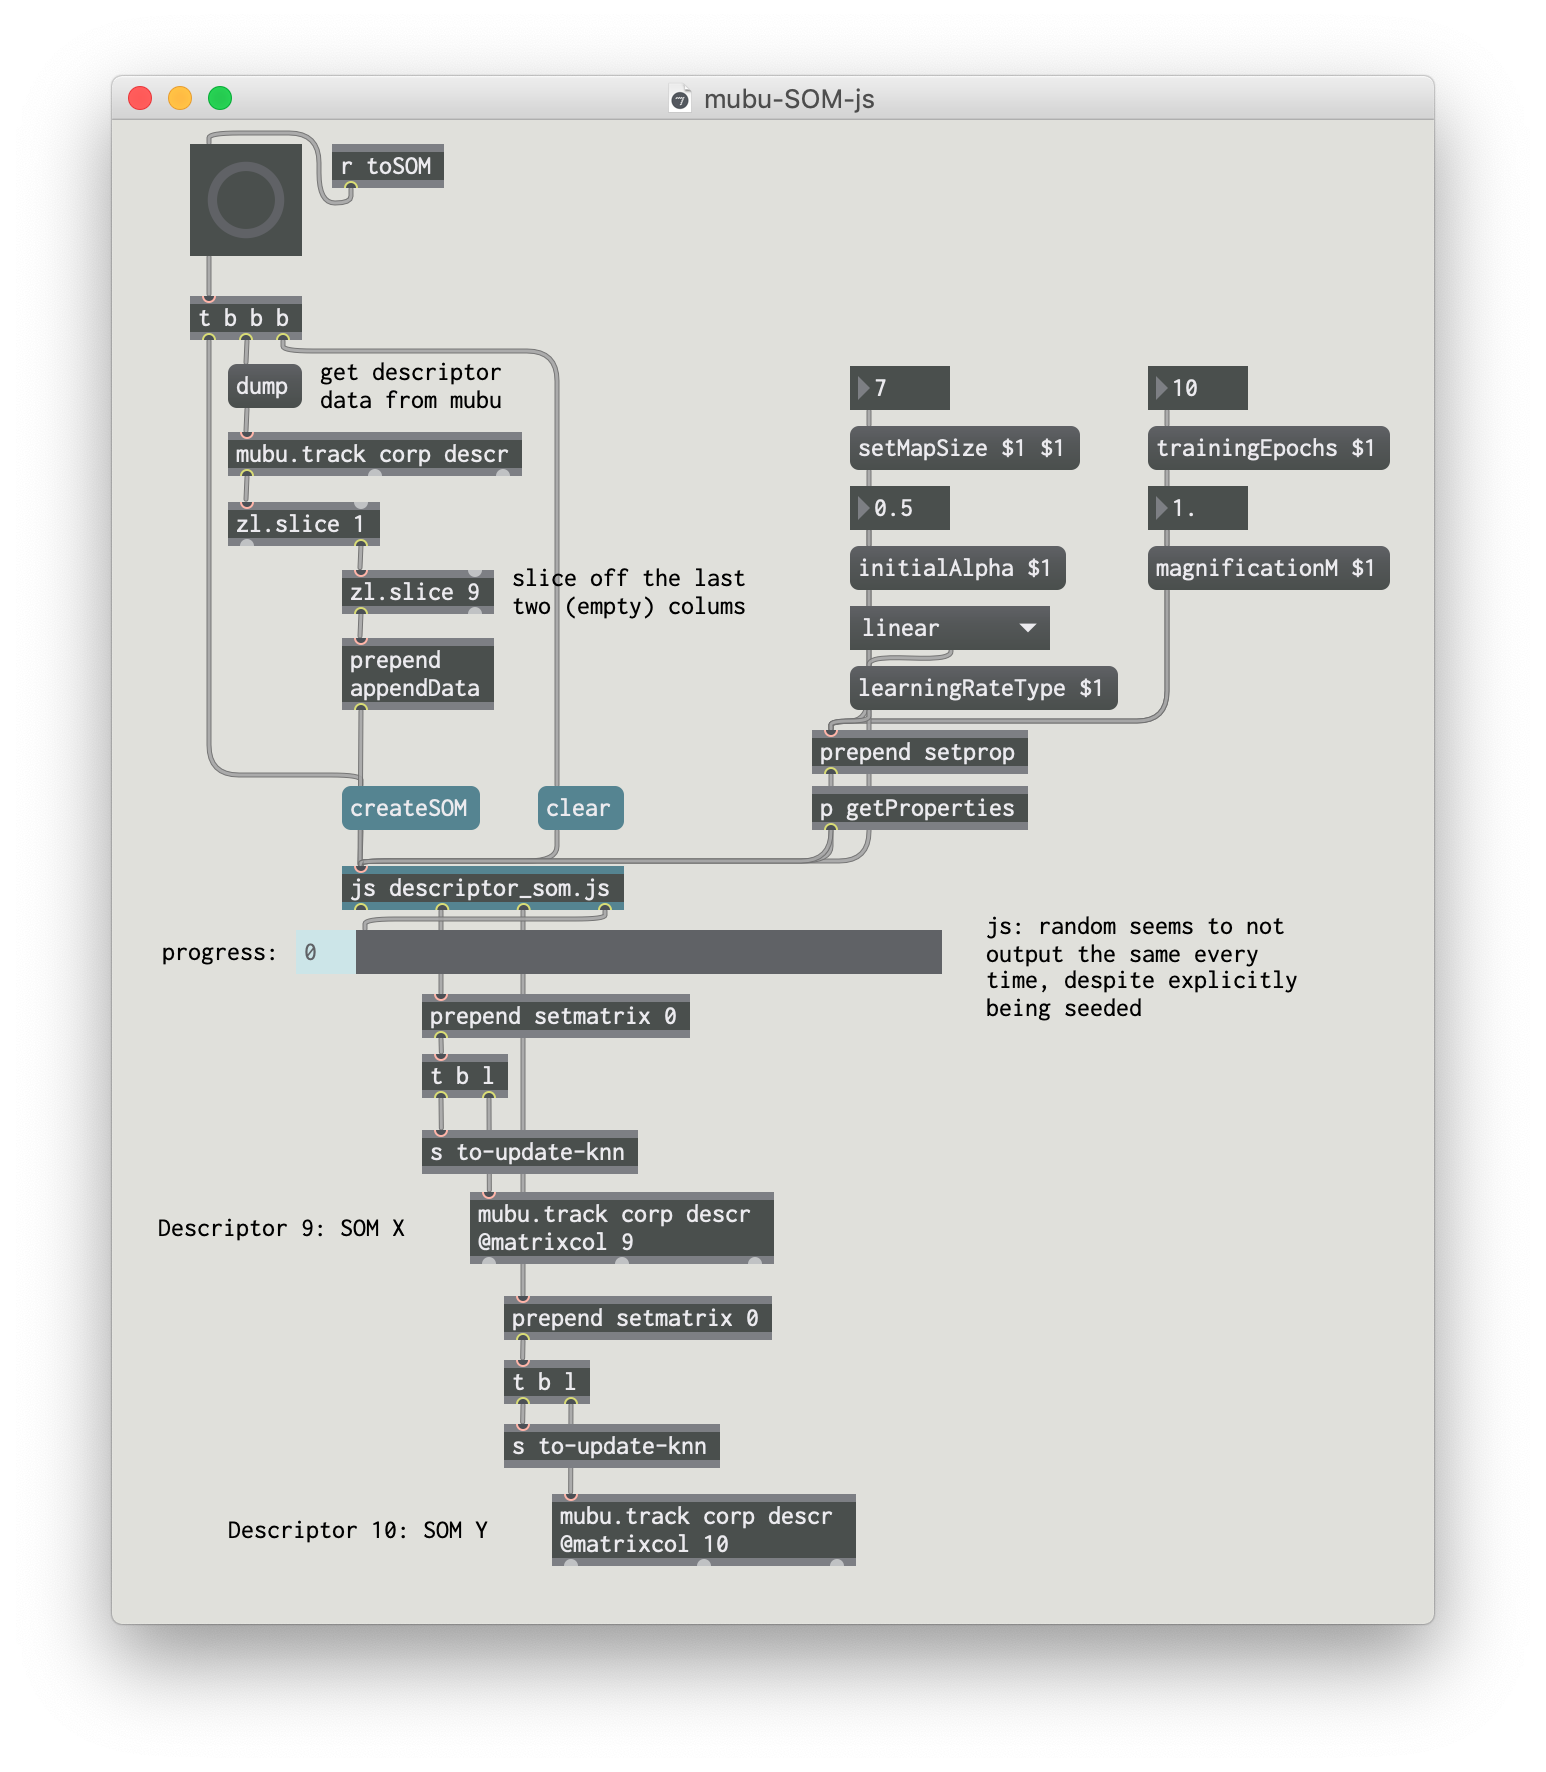
\includegraphics[width=0.8\linewidth, clip]
  {mubu-som-js}
  \caption{mubu-SOM-js}
  \label{fig:mubu-som}
\end{figure}

\begin{figure}[!htb]
  \centering
\begin{subfigure}{0.45\textwidth}
  \centering
  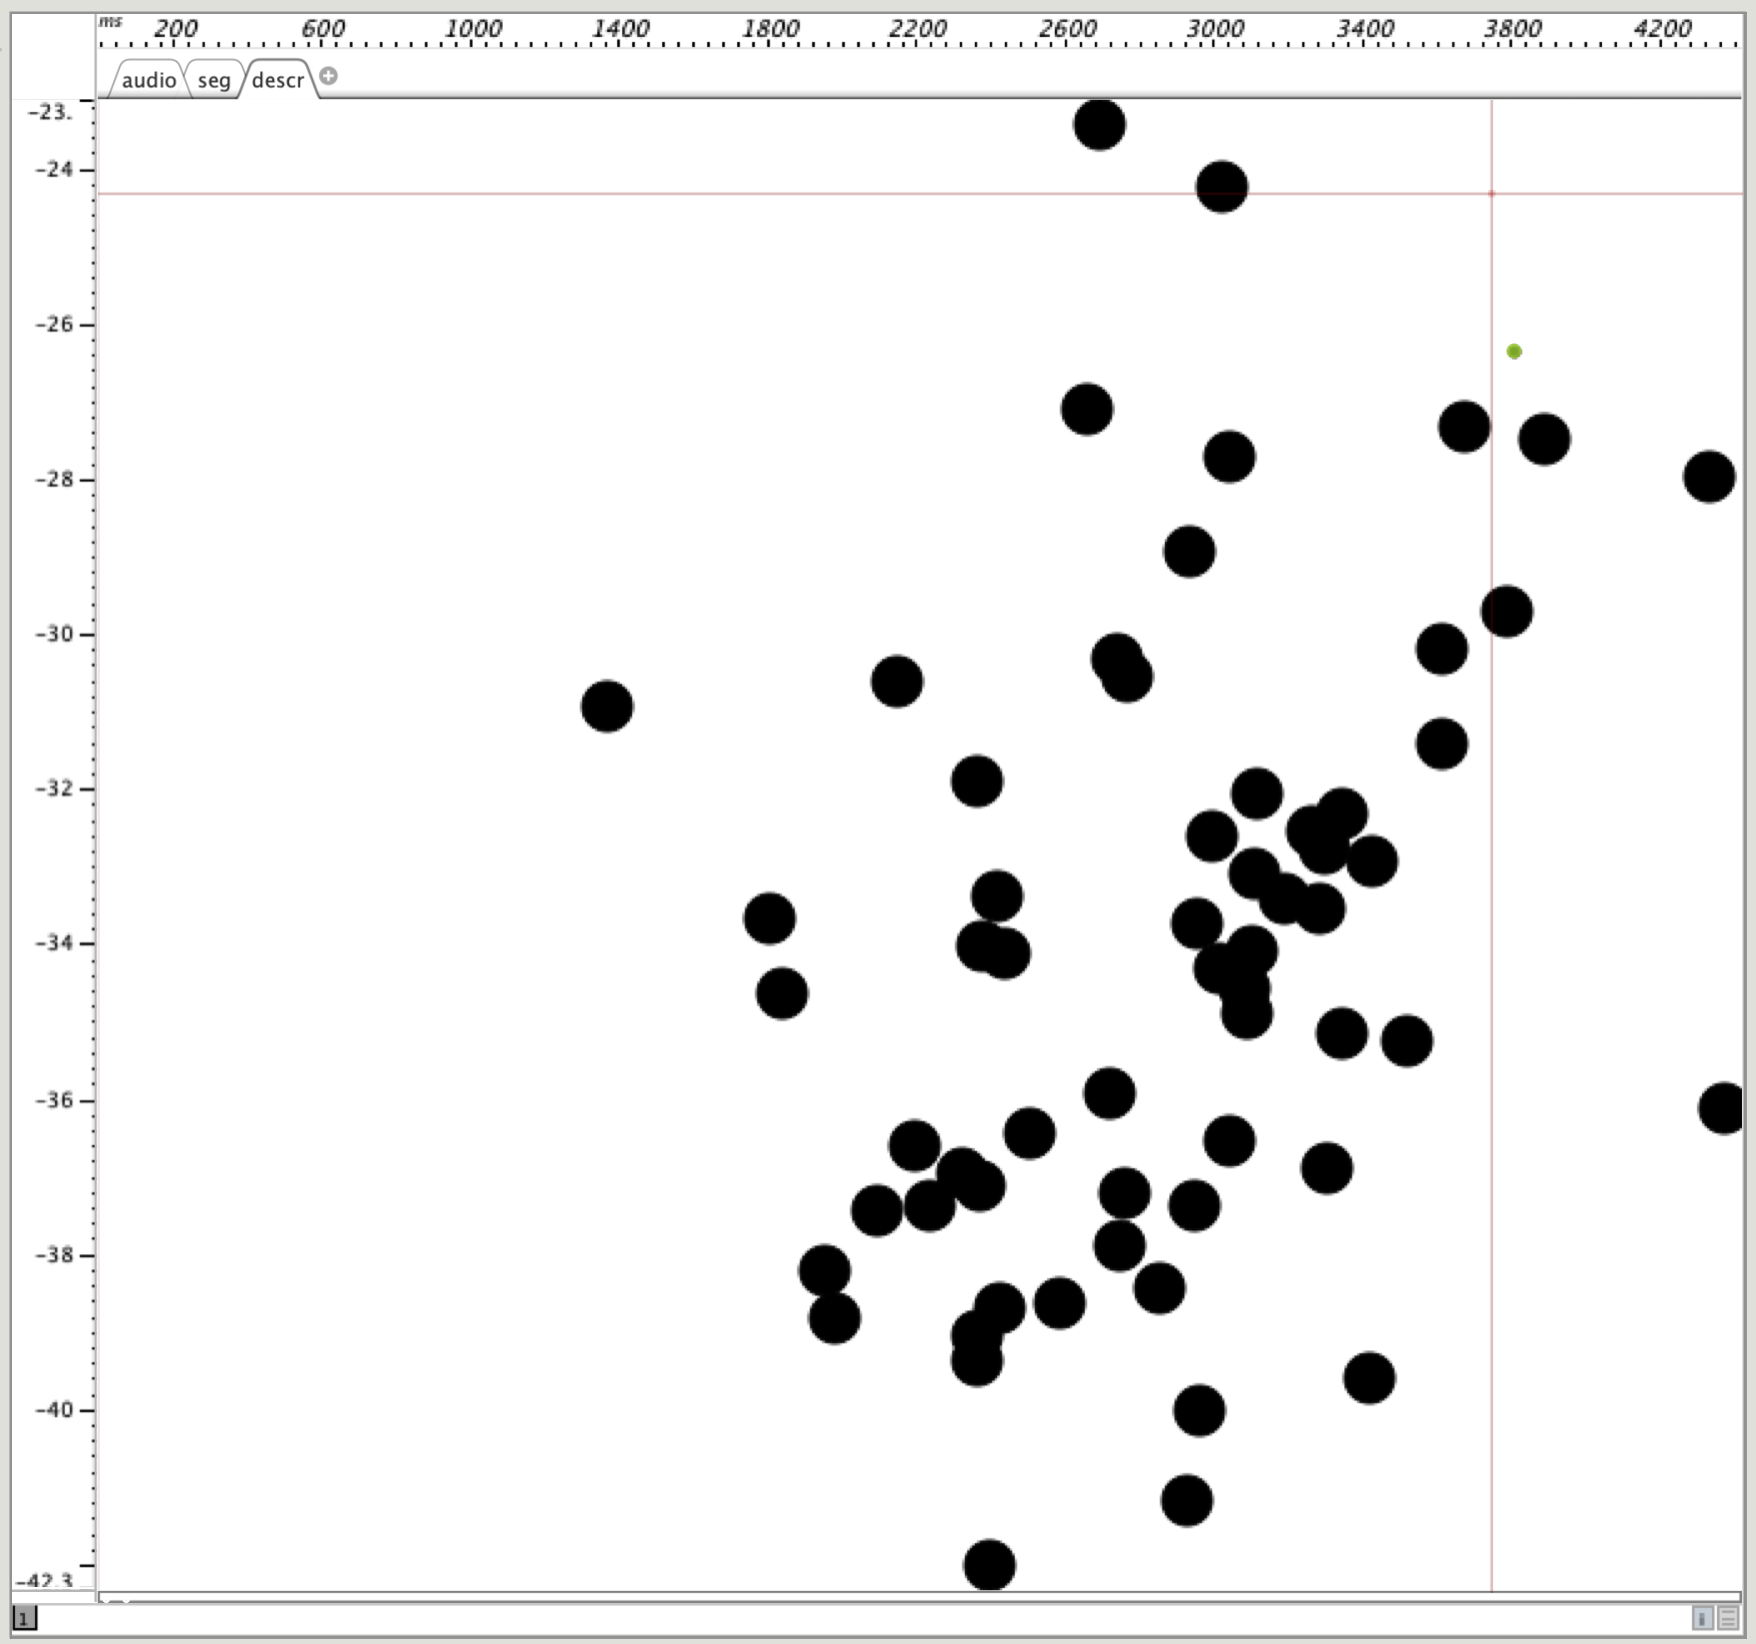
\includegraphics[width=\textwidth]{catart_without_som_centroidVSloudness}
  \caption{}
  \label{fig:catart_no_som}
\end{subfigure}
~
\begin{subfigure}{0.45\textwidth}
  \centering
  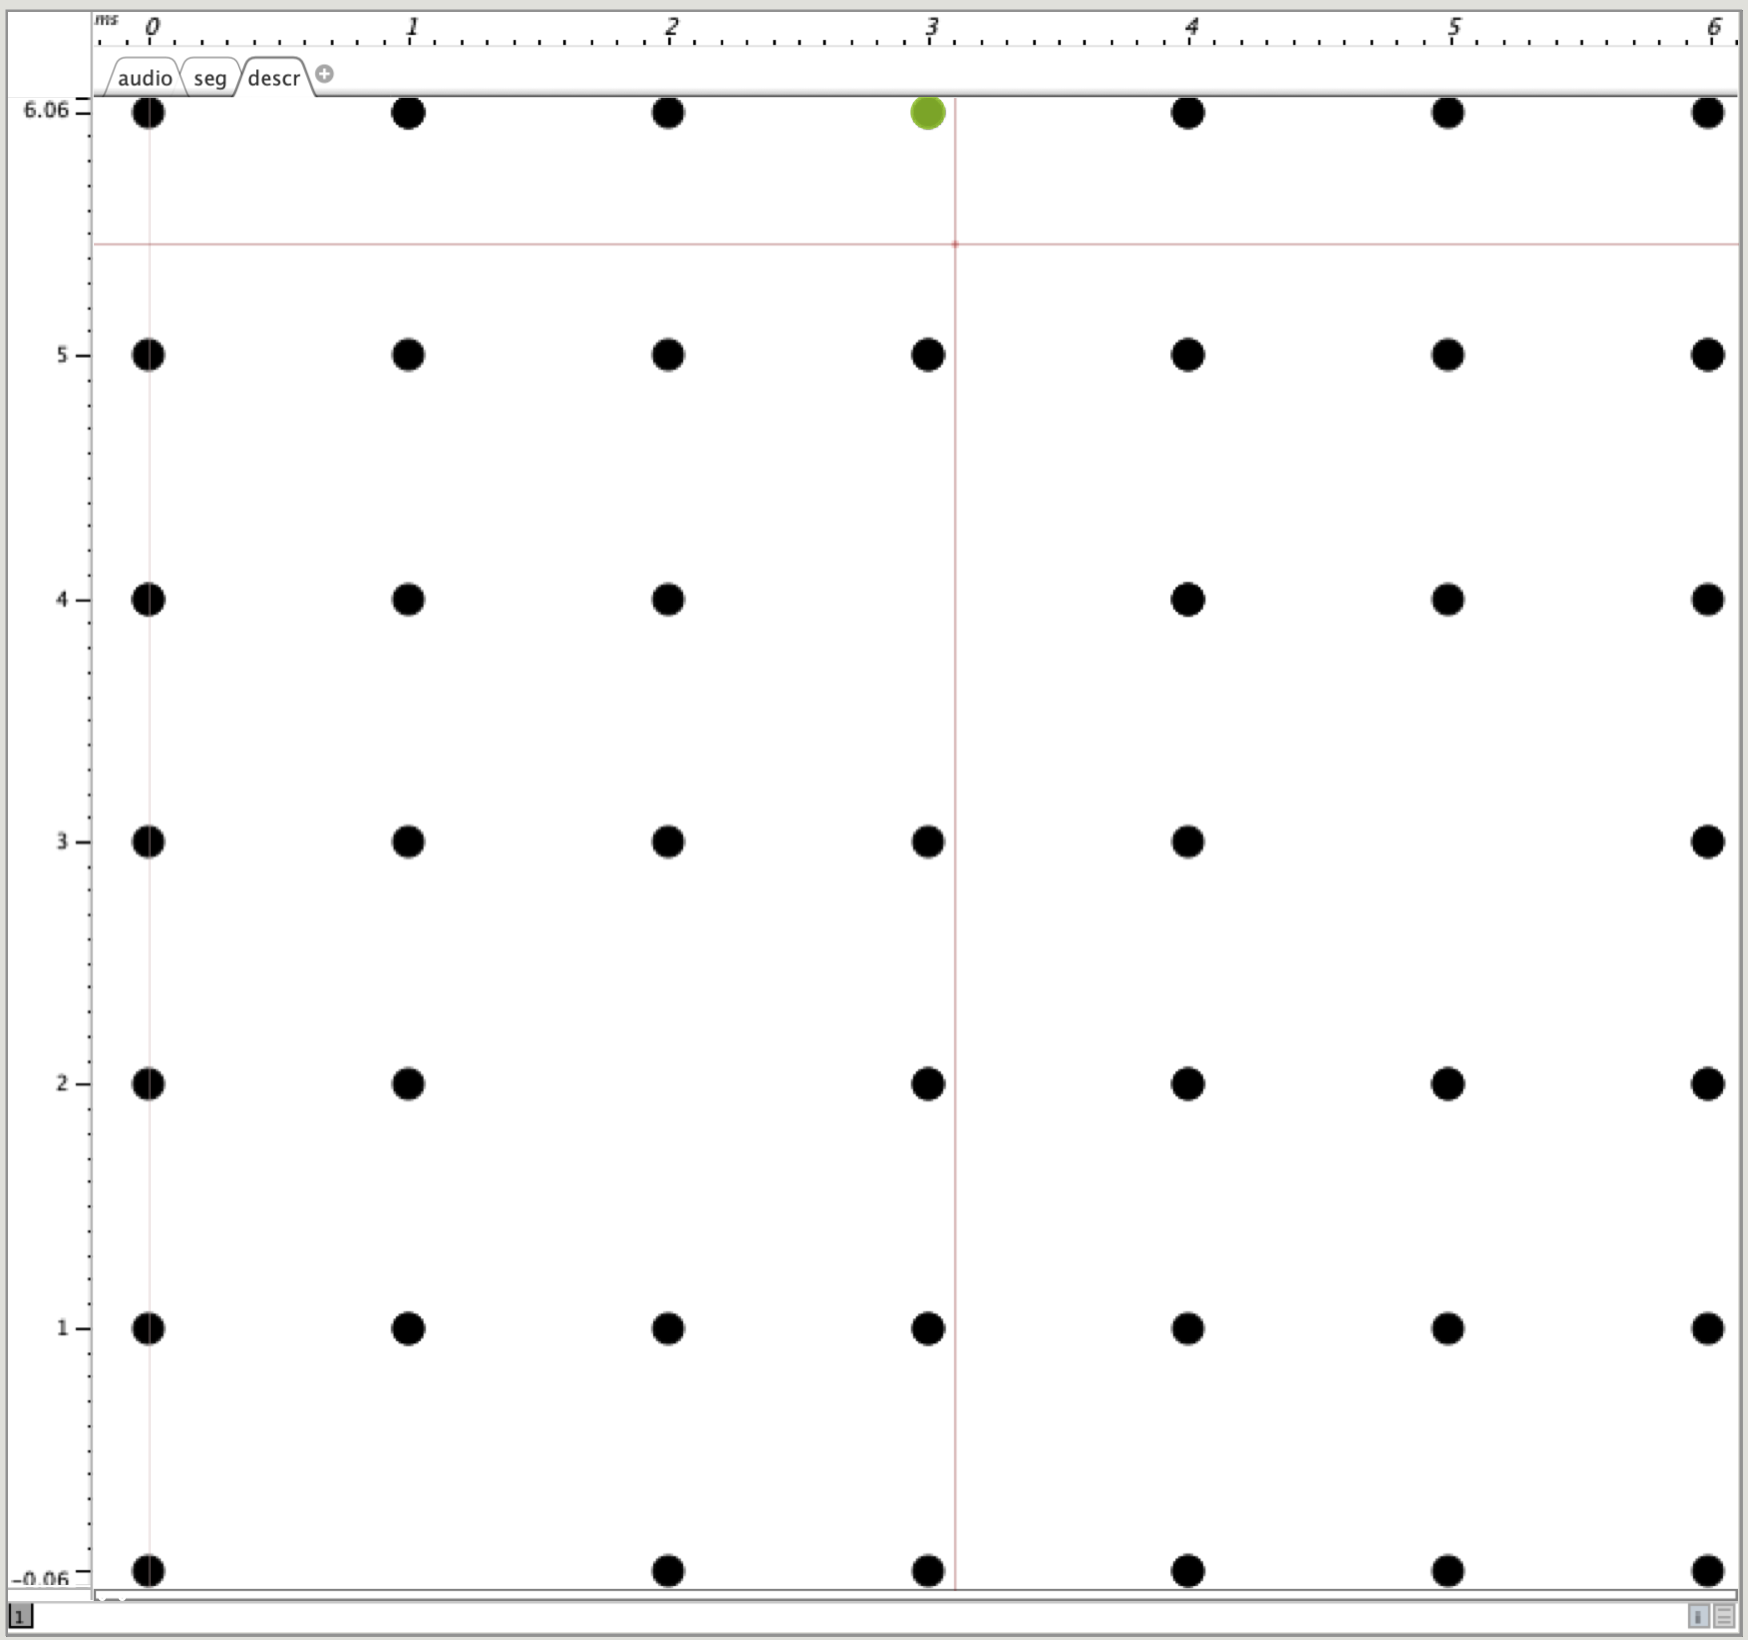
\includegraphics[width=\textwidth]{catart_with_som_no_noise}
  \caption{}
  \label{fig:catart_with_som_no_noise}
\end{subfigure}
\caption[\textit{CataRT}: with and without \gls{som}]{\textit{CataRT} display of
a corpus without \gls{som} (\ref{fig:catart_no_som}, X axis shows spectral
centroid, Y axis shows loudness) and with \gls{som} extension
(\ref{fig:catart_with_som_no_noise}). Each circle represents a sample.}
\label{fig:catart_som_vs_no_som}
\end{figure}

\begin{figure}[!htb]
  \centering
  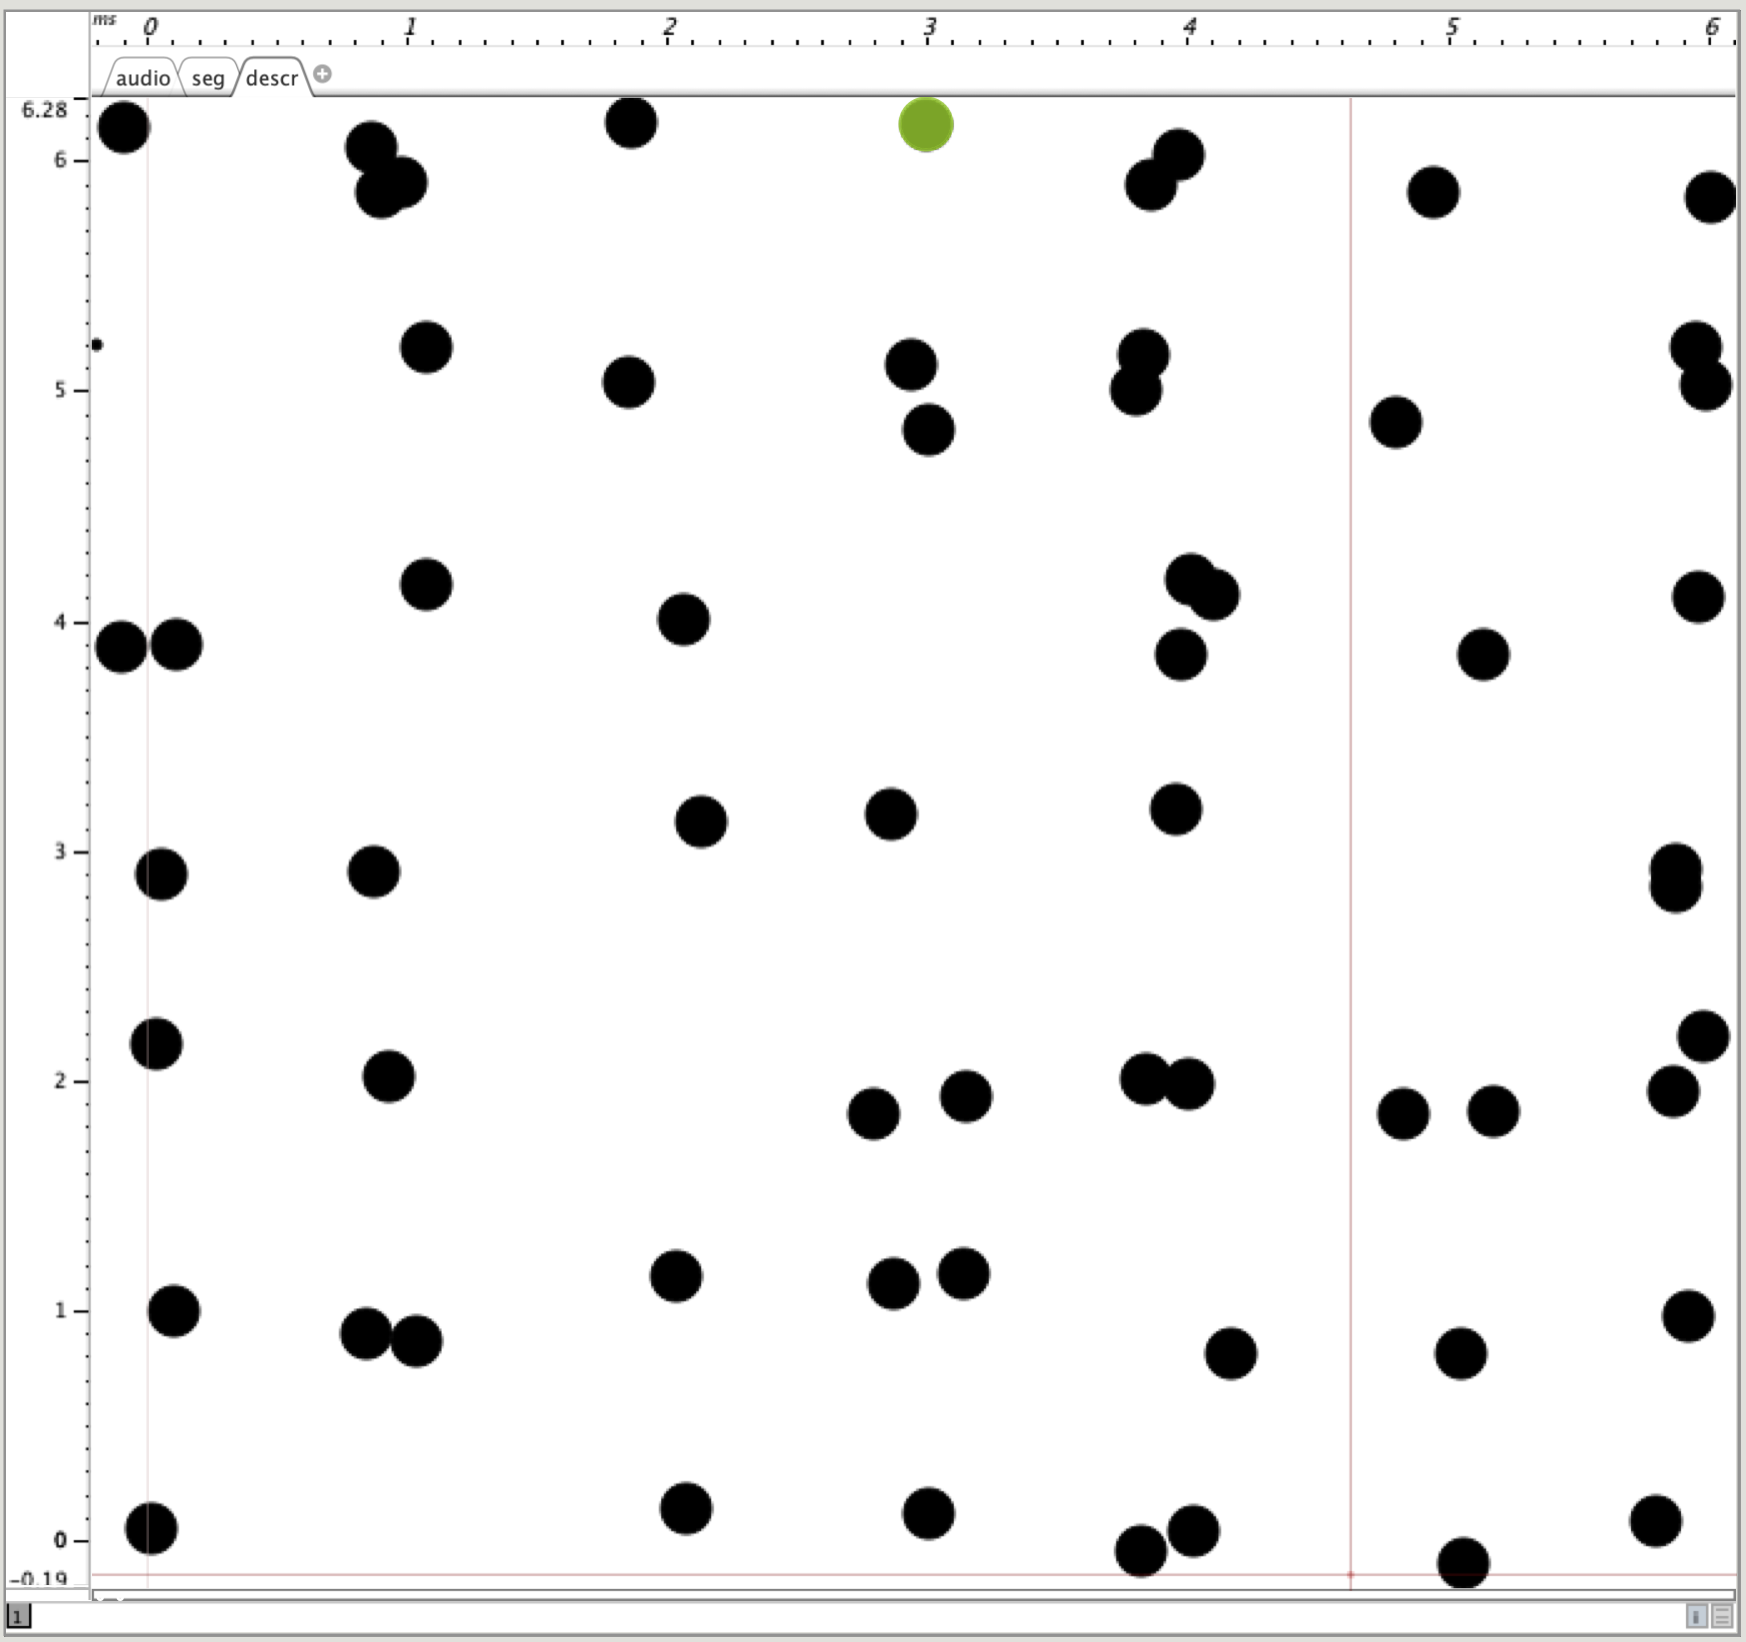
\includegraphics[width=0.45\textwidth]{catart_with_som}
  \caption[\textit{CataRT}: \gls{som} with added noise ]{\textit{CataRT}
  display of a corpus with \gls{som} extension and added noise to
  spatially differentiate samples assigned to the same node. Each circle
  represents a sample.}
  \label{fig:catart_with_som_noise}
\end{figure}


\textit{Catart-by-mubu} uses a
two-dimensional scatter plot interface in which the user can select samples or
grains from the loaded audio corpus (see Figure \ref{fig:catart_som_vs_no_som}).
The spatial position of these sounds in the interface is determined by two audio
features, representing the horizontal and vertical axes, that can be selected by
the user.
The implemented \gls{som} extension gives users the option to choose a
two-dimensional \gls{som} for the spatial organization of the corpus. This
augments the interface in three ways: all analyzed audio features can be
taken into account for the spatial positioning (as opposed to just two at a
time), more of the available interface space is used and additionally the sounds
are spaced in a more even fashion (see Figure \ref{fig:catart_som_vs_no_som}).

\subsubsection{Functionality}
\label{subsubec:mubu-som_functionality}
\textit{Mubu-SOM-js} offers the user simple controls to influence the produced
\gls{som}. These can be set by sending the messages outlined in Table
\ref{table:catart_som_messages} to the \\ \texttt{[js descriptor\_som.js]}
object.

\pagebreak

\begin{table}[!ht]
  \renewcommand{\arraystretch}{1.2}
  \centering
  \footnotesize
  \colorbox{light-bg}{
  \begin{tabular}{ l  l  p{4.2cm}  p{3.1cm}}
    \hline
    \textbf{Message} & \textbf{Type} & \textbf{Description}
    & \textbf{Example} \\
    \hline
    \texttt{createSOM} & n/a & Initiates \gls{som} calculation. &
    \texttt{createSOM} \\
    \texttt{setMapSize \$1 \$1} & Float & Sets size of map.
    & \texttt{setMapSize 7 7} \\
    \texttt{trainingEpochs \$1}
    & Int
    & Defines the length of the training in epochs. One epoch corresponds to
    $n$ iterations of the training algorithm (see section
    \ref{subsubsec:som_math_definition}), where $n$ is the number of samples in
    the corpus.
    & \texttt{trainingEpochs 30} \\
    \texttt{initialAlpha \$1}
    & Float
    & Sets the starting value for the learning
    rate factor $\alpha$.
    & \texttt{initialAlpha 0.5} \\
    \texttt{learningRateType \$1}
    & String
    & Sets the learning rate type (see section
    \ref{subsubsec:som_learning_rates}). It expects a string that is either
    \mintinline{js}{'linear'}, \mintinline{js}{'inverse'} or
    \mintinline{js}{'BDH'}.
    & \texttt{learningRateType 'linear'} \\
    \texttt{magnificationM \$1}
    & Float
    & Sets the magnification control factor $m$ (see section
    \ref{para:alpha_bdh}). Only applies when
    \mintinline[breaklines]{js}{learningRateType === 'BDH'}.
    & \texttt{magnificationM 0.02}
  \end{tabular}
  }
  \caption{mubu-SOM-js: Messages for algorithm control}
  \label{table:catart_som_messages}
\end{table}

\subsubsection{Code Overview}
\label{subsubsec:mubu-som_overview}
The core of the \textit{mubu-SOM-js} Max patch is a JavaScript program (see the
file \texttt{mubu-som-js/descriptor\_som.js}). The choice of programming
language was determined by the fact that \textit{CataRT} is a Max patch and
JavaScript (via the built-in \texttt{[js]} object) can be used to script most
aspects of the Max environment. This JavaScript version of the \gls{som} is in
some ways a port from a first MATLAB implementation of the algorithm that was
developed by the author during an internship at \gls{ircam} in the fall of 2017.
Some aspects of the structure of the presented program are based on the
\gls{som} Toolbox that was developed at Helsinki University of Technology by
\citet{vesanto2000}.

\smallskip

The flow of the script is encapsulated in \mintinline{js}{createSOM()}.
This function calls all other important functions that make up the program, as
can be seen in Listing \ref{lst:mubu-som_create_som}.

\begin{listing}[!htb]
  \begin{mdframed}
    \inputminted[breaklines, numbers=left, firstline=34, lastline=39,
    fontsize=\footnotesize]{js}{../dev/mubu-som-js/descriptor_som.js}
  \end{mdframed}
  \caption{mubu-som-js/descriptor\_som.js: \mintinline{js}{createSOM()}}
  \label{lst:mubu-som_create_som}
\end{listing}

After data normalization and map initialization, \mintinline{js}{trainMap()} is
called, which executes the training procedure by repeatedly calling the function
\mintinline{js}{training()} in an asynchronous background process (see Listing
\ref{lst:mubu-som_training}). For each step of the training phase, all
calculations happen inside \mintinline{js}{trainingStep()}. The most important
part, the updating of node positions on each iteration, is shown in Listing
\ref{lst:mubu-som_node_updates}.


\begin{listing}[!htb]
  \begin{mdframed}
    \inputminted[breaklines, numbers=left, firstline=203, lastline=219,
    fontsize=\footnotesize]{js}{../dev/mubu-som-js/descriptor_som.js}
  \end{mdframed}
  \caption{mubu-som-js/descriptor\_som.js: \mintinline{js}{training()}}
  \label{lst:mubu-som_training}
\end{listing}

\begin{listing}[!htb]
  \begin{mdframed}
    \inputminted[breaklines, numbers=left, firstline=307, lastline=313,
    fontsize=\footnotesize]{js}{../dev/mubu-som-js/descriptor_som.js}
  \end{mdframed}
  \caption[mubu-som-js/descriptor\_som.js: Neuron position updates]
  {mubu-som-js/descriptor\_som.js: Neuron positions are updated in
  \mintinline{js}{trainingStep()}. This Listing implements equation
  \ref{eq:node_update} from Section \ref{subsubsec:som_math_definition}.}
  \label{lst:mubu-som_node_updates}
\end{listing}

\smallskip

After the training phase is finished, the final map is populated by iterating
over all vectors and finding their corresponding best matching units (meaning
that node which is closest), as can be seen in Listing
\ref{lst:mubu-som_find_bmus}. A problem arises when multiple vectors share the
same node as their best matching unit; these vectors will have the same exact
position in the interface with no option to differentiate between them and no
indication of how many vectors reside in that location. To circumvent this
issue, a small amount of random noise is added to each vector's position. This
creates clusters around the exact node position and allows for the individual
circles to be selected. An example of a map with added noise can be found in
Figure \ref{fig:catart_with_som_noise}.

\begin{listing}[!htb]
  \begin{mdframed}
    \inputminted[breaklines, numbers=left, firstline=316, lastline=335,
    fontsize=\footnotesize]{js}{../dev/mubu-som-js/descriptor_som.js}
  \end{mdframed}
  \caption[mubu-som-js/descriptor\_som.js: \gls{bmu} identification]
  {mubu-som-js/descriptor\_som.js: \glspl{bmu} for each vector are
  identified in \mintinline{js}{findBestMatches()}. This Listing implements
  equation \ref{eq:bmu} from Section \ref{subsubsec:som_math_definition}.}
  \label{lst:mubu-som_find_bmus}
\end{listing}

\clearpage

\subsection{SOM Browser}
\label{subsec:implementation_som-browser}

The majority of the work for this thesis consisted of the development of a
standalone application for sample library exploration which we call
\textit{SOM Browser}. A screenshot of the program can be seen in Figure
\ref{fig:som-browser}.

\begin{figure}[!htb]
  \centering
  \makebox[\textwidth][c]{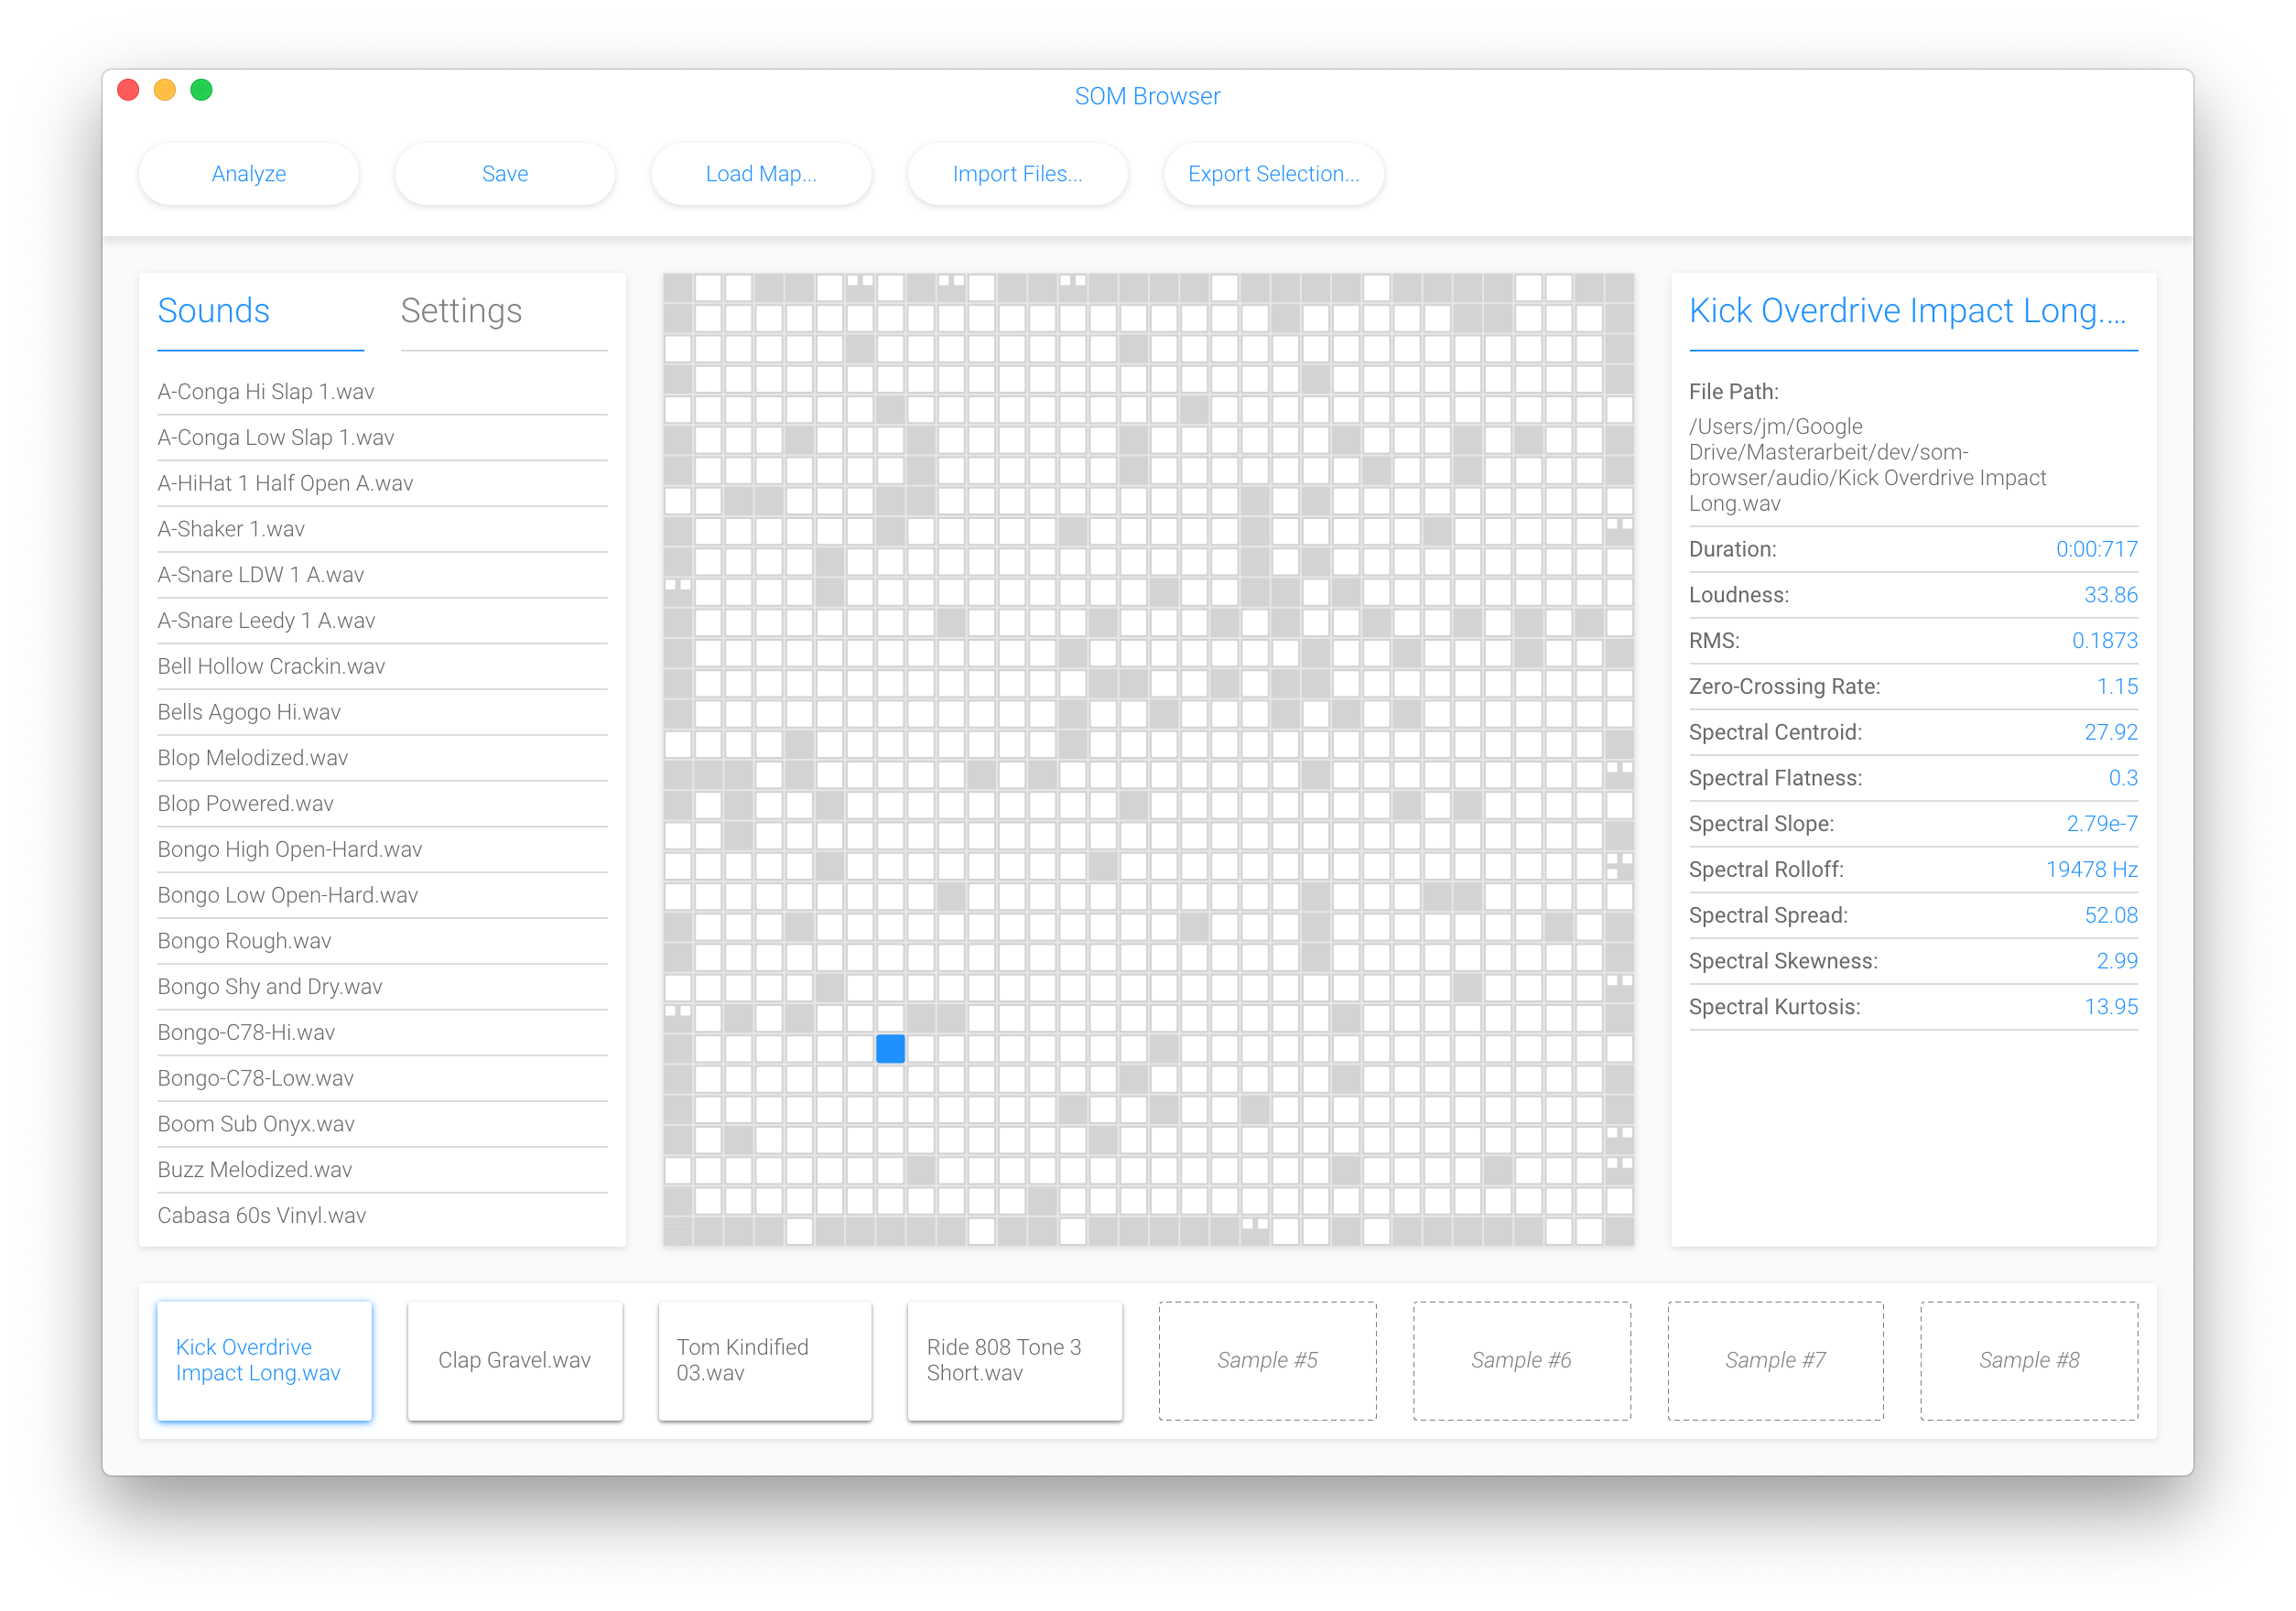
\includegraphics[width=1.2\textwidth]{SOM-Browser}}
  \caption{\textit{SOM Browser}}
  \label{fig:som-browser}
\end{figure}

\textit{SOM Browser} offers users an alternative interface for the interaction
with a folder of audio samples. Instead of the traditional file browser
interface consisting of an alphabetical list of file names, the presented
application offers a spatial map layout of the samples, with the aim of allowing
users a more direct interaction and giving them a quicker overview of the
sounds.

\subsubsection{Functionality}
\label{subsubsec:som-browser_functionality}
\paragraph*{Loading Audio Files}
When launching \textit{SOM Browser}, the application opens with no sounds or map
loaded (see Figure \ref{fig:som-browser_empty}). In order to create a map of
a collection of sound files, the user can go to the menu bar at the top of the
window and click the \textit{"Import Files..."} button to load several audio
files.

\begin{figure}[!htb]
  \centering
  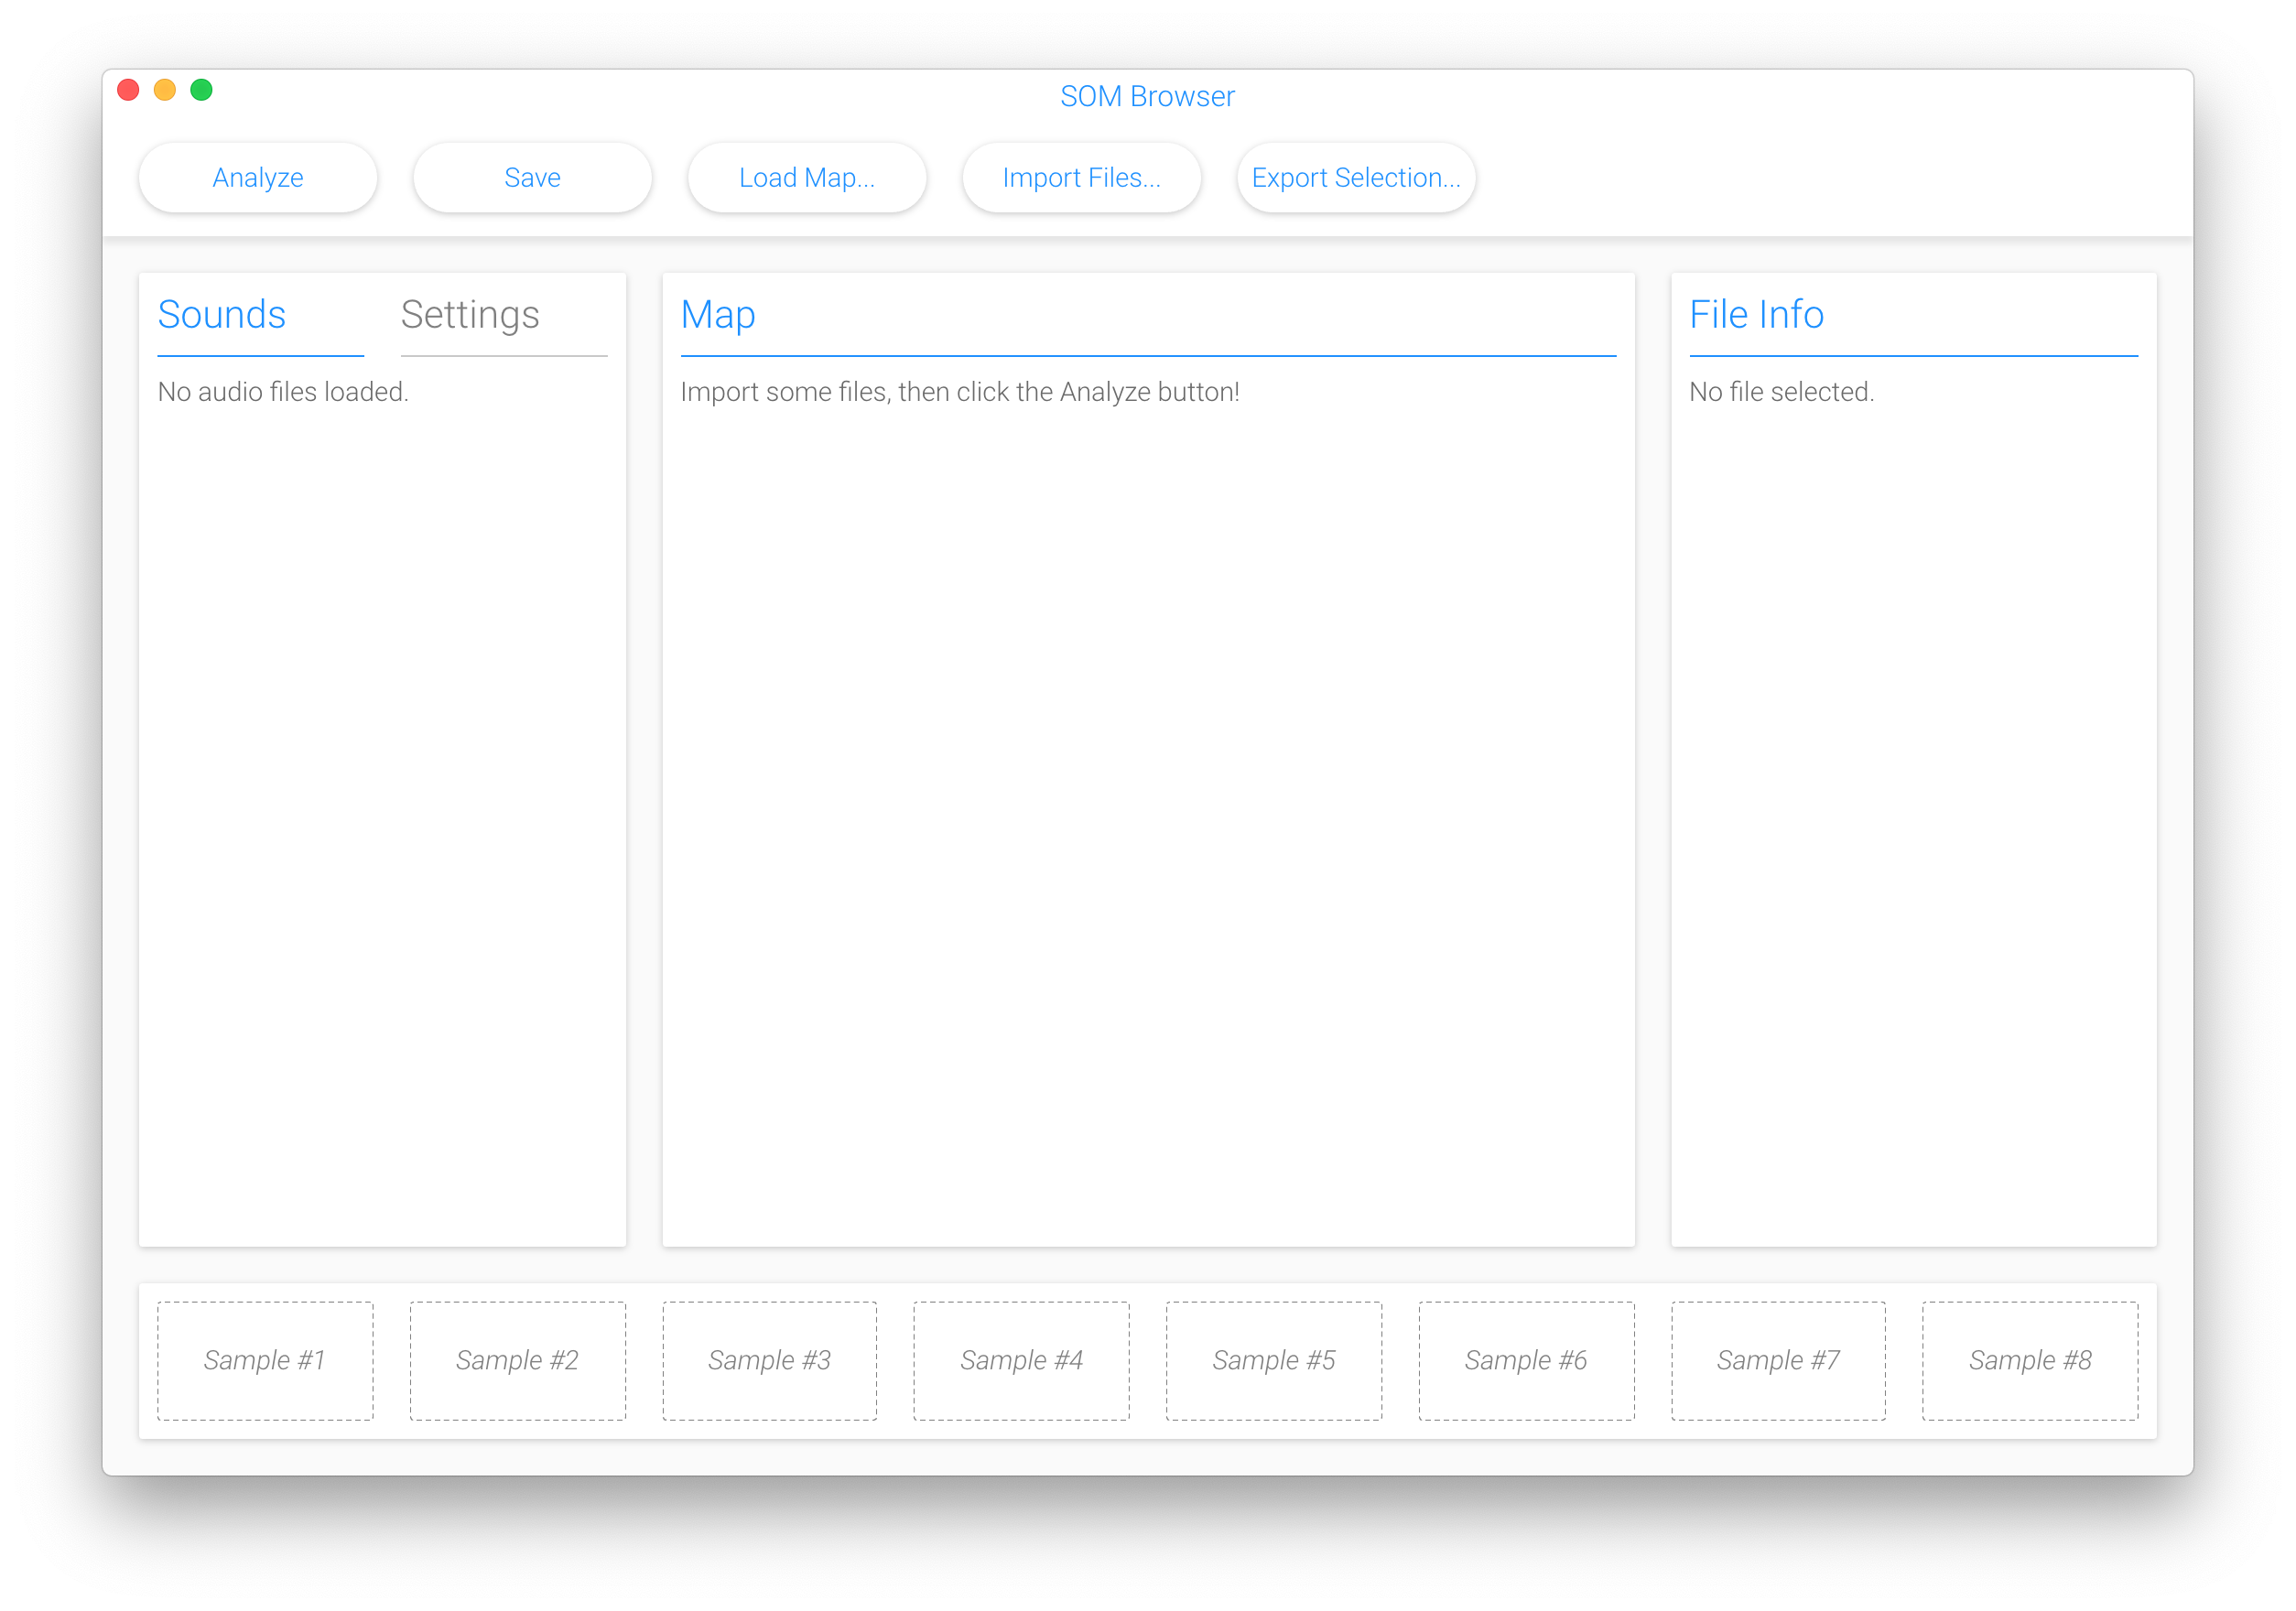
\includegraphics[width=\textwidth]{SOM-Browser_empty}
  \caption{\textit{SOM Browser} without audio files loaded}
  \label{fig:som-browser_empty}
\end{figure}

\paragraph*{Calculating a Map}
Once files are selected, the \textit{Sounds} list on the left side of the
application will be populated. Next, by clicking \textit{"Analyze"}, the program
will start to analyze the audio files in the background, first extracting
audio features (see section \ref{subsec:feature_extraction}) and then using this
information to calculate a \gls{som} using default settings. Alternatively,
some \gls{som} parameters can be altered by selecting the \textit{Settings}
field next to \textit{Sounds} and adjusting the exposed parameters. Depending on
the number of audio files to analyze and the selected training duration, the
algorithm will take a while to process. Training progress is indicated as a
percentage in the central \textit{Map} panel.

\smallskip

\paragraph*{Map Interaction}
Upon completion of the \gls{som} calculation, the \textit{Map} panel will be
populated by a grid of white and grey squares. Each white square represents a
single sound file. All files are loaded into the computer's \gls{ram} for quick
access. Grey squares are empty nodes, meaning nodes to which no sound
files were assigned. Sounds can be played by clicking on the white squares.
They can also be played immediately by holding down the Shift key and hovering
over them.
This allows the user a very fast audition process and makes it
possible to play back many files in fast succession, enabling very quick
browsing of all loaded audio files. When hovering over a square, the
corresponding file name is shown next to the mouse cursor. More detailed
information about the file, including its full path, duration and audio feature
values can be found in the \textit{FileInfo} panel to the right of the map.

\paragraph*{Selecting and Exporting Favorites}
The bottom of the window is taken up by the \textit{Favorites} bar. If a sample
is found on the map that the user would like to save for further usage, they can
drag the square from the map down into one of the slots labeled
\textit{"Sample \#1 - \#8"}. Samples can also be also be played from the
\textit{Favorites} bar by clicking on them. If the user is satisfied with their
selection of samples, they can export the selected \textit{Favorites} (e.g. for
further usage in a \gls{daw}) by clicking on \textit{"Export Selection"} in the
top menu bar. This will open a file dialog window to select a location where the
files should be stored.

\paragraph*{Saving and Loading Maps}
\textit{SOM Browser} also offers the ability to save entire maps to disk for
recall in a later session or import previously stored maps by clicking on the
menu bar buttons \textit{"Save"} and \textit{"Load Map"}.

\subsubsection{Libraries and Frameworks Used}
\label{subsubsec:som-browser_libraries}
Although a desktop application, \textit{SOM Browser} was built entirely using
web technologies, most importantly JavaScript, in order to support multiple
\glspl{os} with minimal effort. A vast variety of libraries and frameworks are
available to use for all aspects of the development process. The following
paragraphs outline the tools chosen for this application and their benefits.

\paragraph*{Electron}
\label{para:electron}
"is an open source library developed by GitHub for building cross-platform
desktop applications with HTML, CSS, and JavaScript. Electron accomplishes this
by combining Chromium and Node.js into a single runtime and apps can be
packaged for Mac, Windows, and Linux" \citep{electron2019}. It offers a variety
of \glspl{api} to offer native menus, interact with the file system and more.
Its \texttt{ipcMain} and \texttt{ipcRenderer} \glspl{api} are used for
asynchronous communication between the \gls{gui} and processes running in the
background.

\paragraph*{React}
\label{para:react}
is a JavaScript library for building user interfaces \citep{react2019}. It
breaks the \gls{gui} into smaller, self-contained units called
\textit{components} that can be independently updated and rendered.

\paragraph*{Web Audio API}
\label{para:web_audio_api}
enables audio processing and synthesis in (web) applications
\citep{webaudio2019}. The use of this \gls{api} makes it possible to write all
audio processing code for the presented work in JavaScript. Its core concept is
the \textit{audio routing graph}, made up of \textit{audio nodes} (simple
building blocks such as an oscillator or a recording). This graph connects
sources to other other nodes (e.g. effects or filters) and finally to an output
destination.

\paragraph*{Meyda}
\label{para:meyda}
"is a Javascript audio feature extraction library. Meyda supports both offline
feature extraction as well as real-time feature extraction using the Web Audio
API" \citep{web:meyda2019}. Its effectiveness has been validated by researchers
at Queen Mary University ("Meyda [...] provide[s] excellent real time feature
extraction tools", \citet{moffat2015}).

\subsubsection{Application Structure}
\label{subsubsec:som-browser_structure}
\textit{SOM Browser} is a \textit{stateful} application, meaning it is designed
to remember user interactions, save its internal data (the \textit{state} of
the application) between interaction steps and allow the storing of state data
between sessions.

\paragraph*{System States}
\label{para:som-browser_states}
Before the start of the development process, a set of system states was designed
to represent the states through which the application is supposed to progress.
These states and their order are shown in Figure \ref{fig:som-browser_states},
giving an abstract overview of the flow of the program. Each panel represents
a state and consists of a title (shown in capitalized words at the top, e.g.
\textit{Map Created}), a method describing a state transition (underscored and
in lower case, e.g. \textit{show map}) and the next state to transition into
(bottom right, marked by an arrow, e.g. $ \rightarrow $ \textit{File Audition}).

\begin{figure}[!htb]
  \centering
  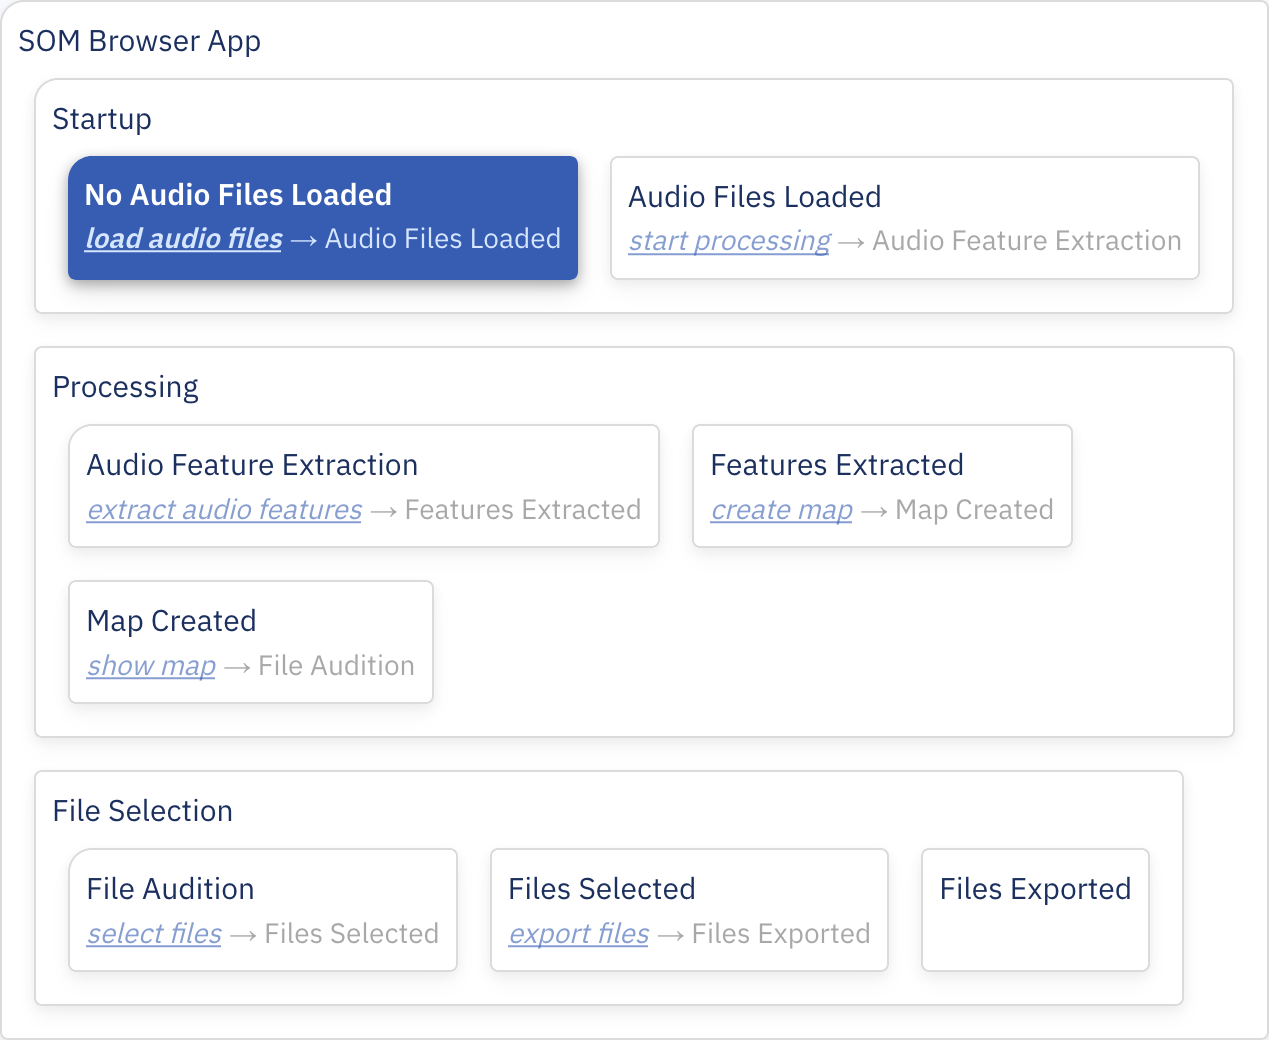
\includegraphics[width=\textwidth]{som-browser_states-sketch}
  \caption{\textit{SOM Browser}: Mock-up outlining system states}
  \label{fig:som-browser_states}
\end{figure}

\paragraph*{Code Overview}
\label{para:som-browser_overview}
\textit{SOM Browser} was developed using the \textit{git} version control
system \citep{git2019} in a repository on GitHub \footnote{\href
{https://github.com/jonasmargraf/som-browser}
{https://github.com/jonasmargraf/som-browser}}.
The very basic structure of the application, in particular the way in which the
Electron and React frameworks interact, is based on a boilerplate project by
Phillip Barbiero \citep{barbiero2017}.

\smallskip

The entry point of any Electron application is the \texttt{main.js} file, which
in the presented work can be found in \texttt{som-browser/src/main.js}.
This file creates an instance of the \mintinline{js}{BrowserWindow} class called
\mintinline{js}{mainWindow} that serves as the single visible application
window. \mintinline{js}{mainWindow} then loads
\texttt{som-browser/src/index.js}, which imports the React library and uses the
React function \mintinline{jsx}{render()} to create the
\mintinline{jsx}{<App />} component, which is defined in
\texttt{som-browser/src/components/App.js}. It serves as a container for the
rest of the application logic and the entire \gls{gui} (see Listing
\ref{lst:som-browser_app_content} and Section
\ref{subsubsec:som-browser_components} for more details).
From here, the structure of the source files branches out into the individual
\gls{gui} elements in \texttt{som-browser/src/components/} and a set of files in
\texttt{som-browser/src/background/} containing the code for audio feature
extraction and \gls{som} calculation.

\subsubsection{Background Processing}
\label{subsubsec:som-browser_background_processing}
Both audio feature extraction and \gls{som} calculation are processing intensive
tasks, therefore it was clear from the beginning of the development stage that
these parts of the application must be separated from the \gls{gui} that the
user interacts with. While it is not possible to build a truly multithreaded
application (due to the fact that the fundamental Node.js framework is single
threaded), one can create separate processes to run different tasks
asynchronously. This is done by creating multiple \mintinline{js}{BrowserWindow}
instances, as each window is running in its own process. These windows can have
their \mintinline{js}{show} flag set to \mintinline{js}{false} in order to hide
them, thereby creating an invisible window for a background process.

\smallskip

\textit{SOM Browser} initiates two consecutive background processes when the
user clicks on \textit{"Analyze"}, one for feature extraction and one that runs
the \gls{som} algorithm. This is handled by the function
\mintinline{jsx}{handleAnalyzeClick()} (found in
\textit{som-browser/src/components/App.js}), which passes the necessary data to
these background processes by calling \mintinline{js}{processFiles(files)} and
\mintinline{js}{createSOM(files, settings)} (see Listing
\ref{lst:som-browser_analyze}). Note the chaining of commands using several
\mintinline{js}{.then()} statements: \textit{SOM Browser} performs asynchronous
operations using the \mintinline{js}{Promise} feature of ECMAScript 2015
\footnote{\href{https://developer.mozilla.org/en-US/docs/Web/JavaScript/Reference/Global\_Objects/Promise}
{https://developer.mozilla.org/en-US/docs/Web/JavaScript/Reference/ \\
Global\_Objects/Promise}}.

\begin{listing}[!htb]
  \begin{mdframed}
    \inputminted[breaklines, numbers=left, firstline=284, lastline=293,
    fontsize=\footnotesize]{jsx}{../dev/som-browser/src/components/App.js}
  \end{mdframed}
  \caption{som-browser/src/components/App.js:
  \mintinline{jsx}{handleAnalyzeClick()} [excerpt]}
  \label{lst:som-browser_analyze}
\end{listing}

\smallskip

The crucial parts of the feature extraction code can be found in Listing
\ref{lst:som-browser_exctract_features}. Since the \gls{som} implementation in
\texttt{som-browser/src/background/calculateSOM.js} is logically identical to
what was previously discussed, we refer to Section
\ref{subsubsec:mubu-som_overview} rather than dissecting the contents of
\mintinline{js}{calculateSOM()} separately.

\begin{listing}[!htb]
  \begin{mdframed}
    \inputminted[breaklines, numbers=left, firstline=66, lastline=91,
    fontsize=\scriptsize]{jsx}
    {../dev/som-browser/src/background/extractFeatures.js}
  \end{mdframed}
  \caption[som-browser/src/background/extractFeatures.js: Audio feature
  extraction]
  {som-browser/src/background/extractFeatures.js: Audio features for
  each sound are extracted in \mintinline{jsx}{extractFeatures()} using the
  \textit{Meyda} library (shown here is an excerpt). Formal definitions for each
  feature can be found in the equations of Section
  \ref{subsec:feature_extraction}.}
  \label{lst:som-browser_exctract_features}
\end{listing}

\subsubsection{User Interface Components}
\label{subsubsec:som-browser_components}
The following paragraphs give an overview of the different React components
that make up the \gls{gui} of \textit{SOM Browser} (refer to Figure
\ref{fig:som-browser} for a screenshot of the program). An outline of the entire
application interface is shown in Listing \ref{lst:som-browser_app_content},
which contains most of the \mintinline{jsx}{render()} function of
\texttt{som-browser/src/components/App.js}, including all components, their
properties and functions.

\begin{listing}[!htb]
  \begin{mdframed}
    \inputminted[numbers=left, firstline=405, lastline=461,
    fontsize=\scriptsize]{jsx}{../dev/som-browser/src/components/App.js}
  \end{mdframed}
  \caption{som-browser/src/components/App.js:
  \gls{gui} Components}
  \label{lst:som-browser_app_content}
\end{listing}

\paragraph*{MenuBar}
\label{para:menu_bar}
is the horizontal element across the top of the application window. It holds
five buttons to perform audio analysis, load and export samples and store and
recall calculated maps.

\paragraph*{FileList}
\label{para:file_list}
is one of two options for content to display in the left panel. It shows a list
of all loaded audio files. Each list element is rendered by a nested
\mintinline{jsx}{FileListItem} component. When clicking an item in the list, the
corresponding map square will be highlighted and the \mintinline{jsx}{FileInfo}
panel on the right will display information about the file.

\paragraph*{Settings}
\label{para:settings}
is the other display option for the left panel. Here, a number of \gls{som}
parameters can be set, similar to the Max messages listed in Table
\ref{table:catart_som_messages}.

\paragraph*{Map}
\label{para:map}
is the main focal point of the application. It displays a grid of grey and white
squares, where each white square represents one sound. The \mintinline{js}{Map}
component is made up of three nested components: \mintinline{js}{MapNode} (the
grey background squares that are rendered first), \mintinline{js}{MapSubNode}
(the white squares representing sounds) and \mintinline{js}{MapLabel} (the
label displaying the name of the sound over which the user is currently
hovering).

\paragraph*{FileInfo}
\label{para:file_info}
is the panel on the right side of the application. It displays details about the
currently selected file, including its path, duration and audio feature values.

\paragraph*{UserSelection}
\label{para:user_selection}
is the horizontal element across the bottom of the application. It consists of
eight instances of the nested component \mintinline{jsx}{UserSelectionSlot},
each representing a spot into which the user can drag a sound to keep as a
reference or for later exporting.

\subsubsection{Algorithm Extension: Forced Node Population}
\label{subsubsec:som_forced_population}

After the \gls{som} algorithm was first implemented in \textit{SOM Browser}, it
became apparent that large parts of almost all created maps remained empty,
which proved frustrating to interact with since these empty areas are
essentially "dead" spots where no sounds are located and no interaction is
possible. A method to counteract this phenomenon was deemed necessary.

\smallskip

In order to avoid "empty" nodes on the \gls{som} - meaning nodes to which no
input vectors are mapped - a post-processing extension was added to the original
algorithm that inverts the mapping process, explicitly iterates over empty nodes
and assigns each one that input vector which is closest. This algorithm
extension, which we call Forced Node Population (\gls{fnp}), executes the
following sequence after the regular \gls{som} has been calculated (refer to
Listing \ref{lst:som-browser_fnp} to see the actual source code implementation):

\begin{enumerate}
  \item Select a random empty node.
  \item Find closest vector for that node and assign it to this node.
  \item Remove this vector from the possible choices.
  \item Repeat.
\end{enumerate}

\begin{figure}[!htb]
  \centering
\begin{subfigure}{0.45\textwidth}
  \centering
  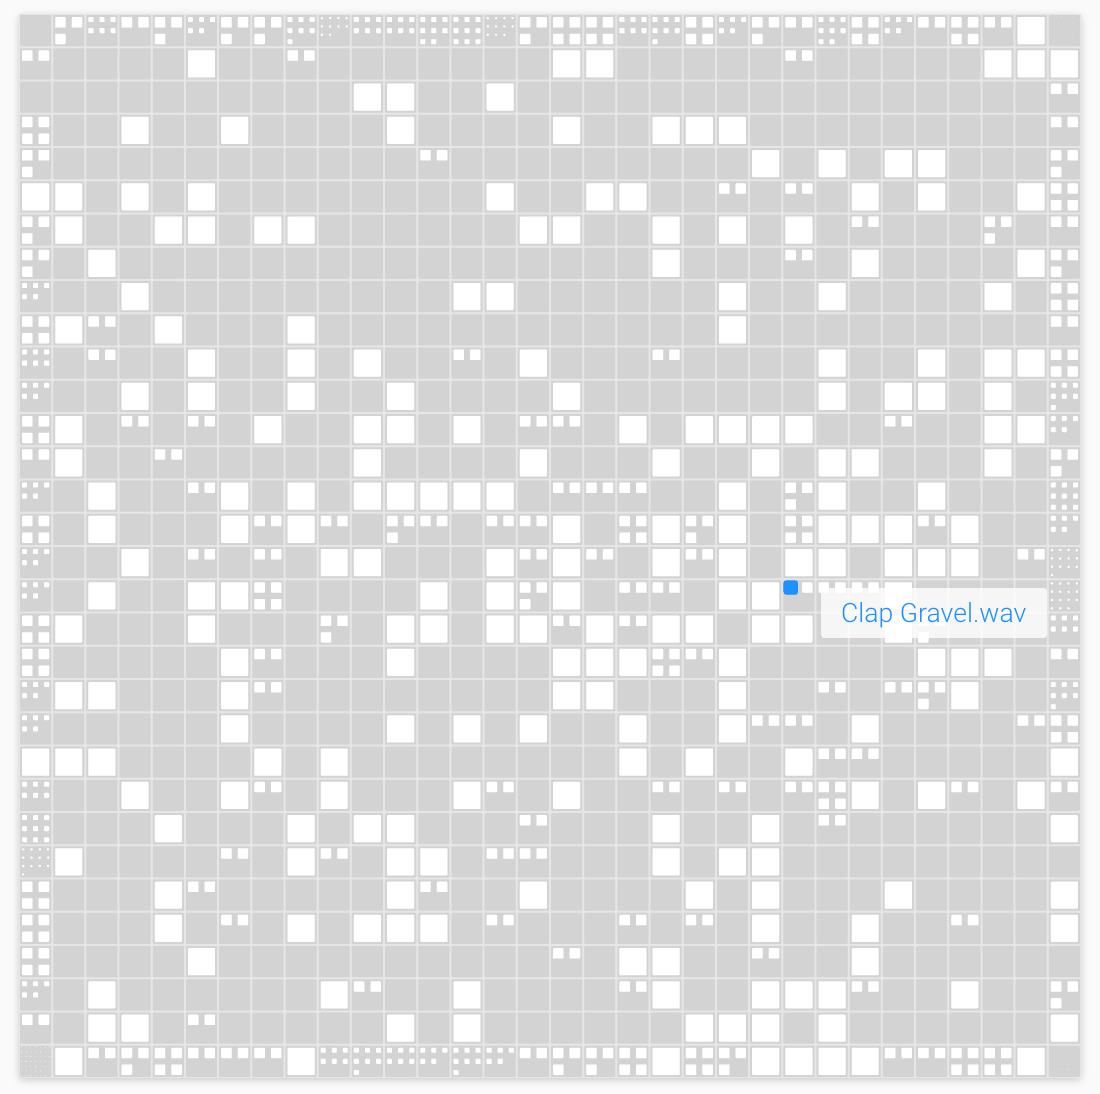
\includegraphics[width=\textwidth]{SOM-Browser_no-FNP}
  \caption{\textit{SOM Browser} without FNP}
  \label{fig:som-browser_no_fnp}
\end{subfigure}
~
\begin{subfigure}{0.45\textwidth}
  \centering
  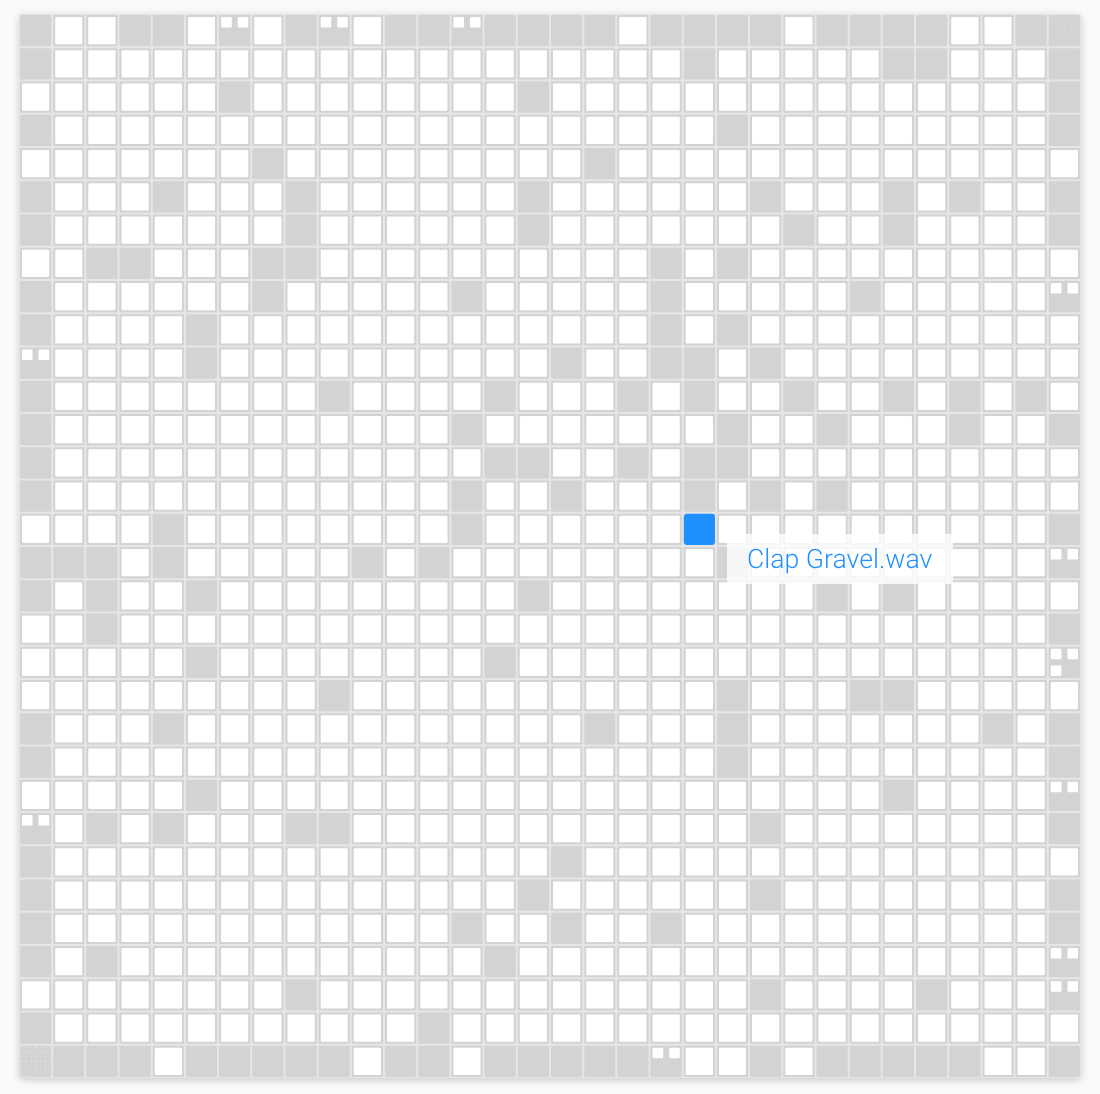
\includegraphics[width=\textwidth]{SOM-Browser_FNP}
  \caption{\textit{SOM Browser} with FNP}
  \label{fig:som-browser_fnp}
\end{subfigure}
\caption[Comparison of maps with (\ref{fig:som-browser_fnp}) and without
(\ref{fig:som-browser_no_fnp}) \gls{fnp}]
{Comparison of \textit{SOM Browser} maps with (\ref{fig:som-browser_fnp}) and
without (\ref{fig:som-browser_no_fnp}) \gls{fnp}. White squares each represent
a sound, while grey squares denote unpopulated (``empty'') nodes. Smaller
squares are used if multiple sounds are assigned to the same node on the map.}
\label{fig:som-browser_fnp_comparison}
\end{figure}

This process is only performed once for all nodes that are empty immediately
after the initial \gls{som} calculation. It is possible that the forced node
population creates new empty nodes, but in order to minimize distortion
introduced by this procedure (see Section \ref{subsec:results_som_metrics}), it
is not repeated. The effect of the \gls{fnp} extension be clearly seen in Figure
\ref{fig:som-browser_fnp_comparison}. For a closer look at the results of this
algorithm extension, please refer to Section \ref{subsubsec:results_final_fnp}.

\begin{listing}[!htb]
  \begin{mdframed}
    \inputminted[breaklines, numbers=left, firstline=358, lastline=394,
    fontsize=\scriptsize]{jsx}
    {../dev/som-browser/src/background/calculateSOM.js}
  \end{mdframed}
  \caption[FNP implementation]{som-browser/src/background/calculateSOM.js:
  The \gls{som} algorithm extension \gls{fnp} (see Section
  \ref{subsubsec:som_forced_population}) is implemented in
  \mintinline{jsx}{populateEmptyNeurons()}.}
  \label{lst:som-browser_fnp}
\end{listing}

\cleardoublepage

% !TEX root = ../thesis.tex

\section{Evaluation}
\label{sec:evaluation}
In order to evaluate the \gls{som} algorithm as implemented in this thesis, as
well as the developed \textit{Som Browser} application as a whole, a two-part
process was employed. First, a set of numerical metrics was selected to quantify
aspects of the algorithm we deem salient when judging its effectiveness for
sound corpus organization. Second, a series of five semi-structured interviews
was designed, conducted and qualitatively analyzed. The following sections go
into detail about the selection of a data set of sound files for the evaluation,
the metrics employed and the design of the interview.

\subsection{Sound Corpus Selection}
\label{subsec:eval_corpus_selection}
A crucial aspect for the evaluation of the work presented in this thesis is the
choice of an appropriate data set of audio files to serve as a prototypical
sound corpus. Ideally, two key conditions should be met by this corpus. It
should be \textit{ecologically valid}, meaning here that it should approximate a
real-world sample library that would actually be used by contemporary music
producers, and it should be a \textit{well-established} data set which has been
validated through use in other research, allowing for direct comparisons between
results. Preferably, something akin to the Giant Steps data sets
\citep{knees2015} for tempo and key detection should be used.
In addition to identifying the aforementioned two conditions, the decision was
made to only select "one-shot" drum and percussion sounds (meaning single
instrument hits, no loops or other longer sounds) in order to evaluate a single,
concrete use case and limit the scope of this evaluation.

\smallskip

Data sets used in previous research vary and it is often not possible to clearly
establish provenance due to insufficient information being given by the authors
(see for example \citet{fried2014} and \citet{shier2017}, two papers which
present important related work but fail to clearly identify the source of their
employed sound files). Two established databases that have been cited in the
literature are ENST-Drums \citep{gillet2006} and the RWC Music Database
\citep{goto2002}. However, neither of these data sets proved appropriate for
this evaluation since they both contain only acoustic source material and,
especially in the case of RWC, largely consist of longer musical passages
instead of the single "one-shot" hits mentioned above.

\smallskip

For the reasons outlined above, we decided to forego the notion that
the selected sound corpus be a data set well-established through previous
research. Because of this, more emphasis is placed on the requirement for
ecological validity. In order to maximize real-world conditions, the sample
library \textit{Drum Essentials} \citep{drumessentials2019} was selected to
serve as a sound corpus for this evaluation. It is a collection of samples
created by the German music software company Ableton AG that is distributed to
owners of the company's flagship product, the \gls{daw} \textit{Ableton Live}
\citep{abletonlive2019}. As part of a commercially available product, this
corpus of sound files does not just approximate a real-world sample library, it
is an actual example of such a library and is, for the purpose of this thesis,
considered representative of sample libraries used in a modern music production
workflow. One additional benefit of using the selected sample library is the
advantage of a single, clearly identifiable source of the data - it is made
available as a professional product by Ableton AG. An alternative approach would
have been to manually select sounds from places like \textit{Freesound.org}
\citep{font2013}, where all files are licensed in a way that makes them free to
use, but their quality is not guaranteed to be consistent, or to scour through
sample libraries shared on various online forums, which brings along issues of
copyright and expired links, making it hard to trace the files' origins.

\smallskip

The \textit{Drum Essentials} collection as distributed by Ableton consists of
1181 one-shot samples, each in a separate audio file, as well as supplementary
content, such as MIDI clips and effects presets. Only the raw audio files are
used in the presented work. These sound files present a mixture of acoustic
and electronic sounds stemming from a variety of drums and percussion
instruments. The library is organized by instrument group, of which there are
17 in total. The names of these groups, as well as the number of sounds per
group can be found in table \ref{table:drum_essentials_counts}. Some sound files
appear in more than one group. These duplicates have been removed, so that every
sound only appears once throughout the entire data set. The remaining number of
sound files is 1081.

\renewcommand{\arraystretch}{1.2}

\begin{table}[!ht]
  \renewcommand{\arraystretch}{1.2}
  \centering
  \textbf{Drum Essentials} \\ [3mm]
  \footnotesize
  \rowcolors{2}{table-bg-one}{light-bg}
  \begin{tabular}{ l c }
    \hline
    \textbf{Instrument Category} & \textbf{Count} \\
    \hline
    Bell & 19 \\
    Bongo & 6 \\
    Clap & 71 \\
    Conga & 27 \\
    Cymbal & 54 \\
    Electronic Percussion & 49 \\
    FX Hit & 64 \\
    Hihat & 167 \\
    Kick & 166 \\
    Misc. Percussion & 64 \\
    Ride & 40 \\
    Rim & 65 \\
    Shaker & 39 \\
    Snare & 181 \\
    Tambourine & 23 \\
    Tom & 138 \\
    Wood & 8 \\
  \end{tabular}
  \caption[\textit{Drum Essentials}: Instrument category counts]
  {Shown are sound file counts per instrument category of the
  \textit{Drum Essentials} sample library.}
  \label{table:drum_essentials_counts}
\end{table}

\subsection{Metrics for SOM Analysis}
\label{subsec:eval_som_metrics}
The optimal \gls{som} for a given sample library should represent the input data
with minimal distortion. Samples should be mapped evenly to the nodes and all
areas of the map should be populated to maximize the usefulness of the
interface space used.

\smallskip

In order to evaluate the \glspl{som} created using the SOM Browser application
and the \textit{Drum Essentials} test data set, three core metrics are used:
quantization induced by the \gls{som}, map emptiness, and the ratio between
nodes and their assigned vectors. These metrics and the motivation behind them
are outlined further in the following paragraphs.

\subsubsection{SOM-Induced Quantization}
\label{subsubsec:som_quantization}
Fundamental to the \gls{som} principle is the idea of mapping vectors to their
corresponding \glspl{bmu}, those nodes that are closest to them (see section
\ref{subsec:som}). Several vectors can be assigned to one node - this can also
be thought of as a quantization process, where the magnitude of the difference
between the positions of vector $ x_t $ and node $ m_c $ is the quantization
error $ \Delta_t $ for that vector:

\begin{equation}
  \Delta_t = || x_t - m_c ||
\end{equation}

As a metric for the \gls{som}, the quantization errors for all vectors can be
averaged, as well as their distribution examined. In order to maximize
information preservation, quantization errors should be minimized.

\subsubsection{Vector-Node Count}
\label{subsubsec:vector_node_count}
A second metric that was devised in order to quantify \gls{som} quality is the
count $ C_i $ of vectors $ x_1, ... , x_n $ mapped to a node $ m_i $ and
subsequently the distribution of those counts across the map. Ideally, this
distribution should look like a single, narrow spike - meaning that (almost) all
nodes have about the same number of vectors assigned to them, resulting in an
even distribution of sounds across the SOM Browser map interface. \gls{som}
parameters should be chosen to approximate a uniform vector-node count for all
nodes.

\subsubsection{Map Emptiness}
\label{subsubsec:map_emptiness}
Another relevant aspect of the created \glspl{som}, and the third metric
employed here, is how much of the map remains "empty", meaning how many nodes
were not assigned any vectors. We define this "map emptiness" metric $ ME $ as
the number of nodes $ m_1, ... m_n $ whose vector-node count $ C_n = 0 $ (see
section \ref{subsubsec:vector_node_count}), divided by the total number of nodes
$ m_i $. For the purpose of making optimal use of the space alloted to the map
in the SOM Browser \gls{gui}, emptiness should be minimized so that users
encounter the least amount of "blind spots" possible.

\subsubsection{Influence of Forced Node Population}
\label{subsubsec:eval_fnp_influence}
Since the concept of Forced Neuron Population is an addition to the \gls{som}
algorithm introduced in this work (see section
\ref{subsubsec:som_forced_population}), its influence on the \gls{som} should
also be evaluated. Therefore, the aforementioned metrics were calculated
both with and without \gls{fnp}.

% \subsection{Online Sound Similarity Survey}
% \label{subsec:evaluation_survey}
% Maybe not even do this bit???

\subsection{Semi-structured User Interviews}
\label{subsec:evaluation_interviews}
In order to evaluate the \textit{SOM Browser} application prototype presented in
this thesis, five semi-structured interviews with working audio professionals
were conducted. These interviews were conducted by the author and consisted of a
set of questions as well as observed user interaction with the prototype
software. For this evaluation, a guide including questions outlining the
structure of the interview as well a set of ratings scales was created. Subjects
were asked about their experience with sample libraries and their current
workflow, and to interact with a sample library in a file browser environment as
well as using the \textit{SOM Browser} software. Audio from the conversations
was recorded and subsequently qualitatively analyzed.

\subsubsection{Motivation to Conduct Interviews}
\label{subsubsec:interview_motivation}
This evaluation procedure entails two aspects, namely a semi-structured
interview series and a qualitative analysis of the collected responses. The
decision to conduct qualitative interviews stems from the exploratory nature of
the presented work. In order to assess the merit of the developed interface in
its present state, direct feedback from potential users was sought, which
\citet{lazar2017} refers to as "fundamental to human-computer-interaction (HCI)
research" (see \citet[p.187]{lazar2017}). But the motivation for a direct
conversation with users was not only to evaluate the presented interface
proposition, but also for these interviews to serve as an exploration of users'
current situation, to hear about their own experience of it and to see what
advantages and shortcomings they identify in their present workflows. In short,
these interviews were motivated by a desire to gain some understanding of the
complex situation that is sample library interaction in a music production
environment and to gauge initial reactions to the developed prototype
alternative. The semi-structured approach was chosen in order to be able to
react to interviewees' responses more freely and allow the interviewer to ask
follow up questions when deemed necessary. Naturally then, the gathered
responses cannot simply be quantified, which makes a qualitative approach to
their analysis a fitting choice.

\smallskip

There are of course downsides to the chosen approach. Conducting
interviews is time-consuming, as it has to be done on a one-on-one basis and
often (as in the case of this work) in person. After the interview is over,
additional time and effort goes into transcribing and annotating the responses.
This severely limits the number of participants that can feasibly be recruited
for a study, as is evident by the small number of five participants here.
\citet{lazar2017} identifies another disadvantage of interviews: "[...] data
collection that is separated from the task and context under consideration [...]
suffer[s] from problems of recall. [...] [I]t is, by definition, one step
removed from reality" \citep[p.188ff.]{lazar2017}. Because of this, we follow
the authors' suggestion of combining the interview with user observation.

\subsubsection{Interview Subject Selection}
\label{subsubsec:subject_selection}
The SOM Browser application is not aimed at the general population. Instead, it
has been designed for specialized users that work in modern music production, as
they constitute the potential future user base of an application like the one
presented here.

\smallskip

In order to increase the validity and relevance of potential subjects'
responses, the decision was made to interview only working professionals for
this evaluation and to not include hobbyists or people without any experience in
music production.

\smallskip

Subjects were recruited by inquiring about qualified candidates (in other words,
people working professionally in modern music production) in the wider circle of
acquaintances of the author. No compensation was offered and only sparse
information about the nature of the research was given beforehand in order to
minimize the possibility of instilling biases in subjects. Most importantly,
subjects were asked to participate in an interview about sample library
organization, but were not told that they would be shown software developed by
the author.

\subsubsection{Informed Consent Form}
\label{subsubsec:consent_form}
For the purpose of documenting participants agreement to be interviewed, an
informed consent form was created for the interview series. This document
outlines basic information about the purpose and content of the interview and
its duration. It also lists all data that will be collected and explains the
procedure used for data anonymization in order to protect subjects' privacy.
Lastly, it informs participants of their rights to withdraw their consent to the
usage of their data for research purposes and have it erased. This form was
based on a template provided by the ethics board of \gls{tu-berlin} on
their website \citep{web:ethics2019}. The form used by the author can be found
in
% TODO
XXX REF APPENDIX HERE XXX.

\subsubsection{Test Subject Code Design}
\label{subsubsec:subject_code}
To ensure proper data anonymization, a test subject code was used. This code
is comprised of a series of letters and numbers and was created at the beginning
of the interview by the subjects themselves according to a set of instructions.
All data and responses of the subjects were directly labelled with this code, so
that individuals' names were never used. This code design procedure was again
based on a template by the ethics board of \gls{tu-berlin} and can be found
on the same website as the information concerning consent forms
\citep{web:ethics2019}. The instruction sheet that was distributed to subjects
can be found in
% TODO
XXX REF APPENDIX HERE XXX.

\subsubsection{Interview Structure}
\label{subsubsec:interview_structure}
The guide developed for this interview can be found in
% TODO
XXX REF APPENDIX HERE XXX
It outlines a three part structure: first, some general questions about
subjects' usage of sample libraries are posed. Second, some guided interaction
with a predetermined sample library in a traditional file browser structure on a
computer follows. In the third section, the SOM Browser application is finally
introduced and subjects are asked to use it and describe their impression of it.

\subsubsection{Question Design}
\label{subsubsec:question_design}
The general composition employed for most questions is twofold, combining
closed- and open-ended approaches: first,
participants are asked to give a rating on a predefined scale (see
\ref{subsubsec:ratings_scales} below).
Then, participants are free to elaborate on their answer and explain their
rating. If they don't initiate this themselves, a follow-up question along the
lines of "Could you tell me why you chose this rating?" is asked.

\subsubsection{Selection of Ratings Scales}
\label{subsubsec:ratings_scales}
In order to record subjects' ratings, 6 point Likert scales were used (as is
common in \gls{hci} research, see \citet[p.31, p.93]{lazar2017}). The difference
between even and uneven anchor counts in Likert scales lies in the presence (in
the case of uneven anchor counts) or lack (for even counts) of a "neutral"
middle option. Choosing scales without neutral mid-points was motivated by a
desire to encourage subjects to make a definite choice with regard to their
rating. For a short look at the effects of eliminating the mid-point, see
\citet{garland1991}.
\smallskip
The scales presented to subjects were explicitly labeled textually instead of
numerically. The anchor points were designed using two polar adjectives (such as
"positive" and "negative") and a consistent, three-tiered set of adjective
qualification with "very" marking the strongest option, followed by the
adjective without qualifier and then "somewhat" as the weakest variant. The
resulting scale for a positive/negative rating is composed of the following
anchors: very positive, positive, somewhat positive, somewhat negative,
negative, very negative. The selection of these qualifiers and appropriate
anchors in general was inspired partially by \citet{vagias2006}. The full set of
scales used for the conducted interviews can be found in
% TODO
XXX REF APPENDIX HERE XXX.

\subsubsection{Questions Used}
\label{subsubsec:questions_used}
In section 1, which serves as an introduction for the interviewee, general
administrative requirements such as the signing of the consent form and a
topical introduction of the research are taken care of. This is then followed
by two simple Yes/No questions to establish whether the subject works with
third-party and/or personally created sample libraries (see questions 1.1 and
1.2).

\bigskip

Section 2 begins with a presentation of the \textit{Drum Essentials} sample
library to the subject. This presentation includes the information that it is a
library of drum samples that consists of around 1000 sound files which are
organized in subfolders according to the respective instrument, such as kick
drum, snare drum, hi-hat, and so forth. The interviewee is invited to explore
the sample library using the laptop that it is being presented on.

\par
Then, in
question 2.1, subjects are asked to describe how to approach familiarizing
themselves with the provided sample library in order to use its contents in a
hypothetical work project of theirs.

\par
Question 2.2 follows this up with a
request for a rating of the subject's level of satisfaction with the workflow
that they outlined.

\bigskip

In the third and final section of the interview, the SOM Browser software is
introduced to participants. At first, a general overview of the interface is
given, in which the interviewer mentions the map layout in the middle (without
explaining the nature of its organization), the file list on the left, the file
info panel on the right and the favorites bar at the bottom.

\par
The subject is
then asked to try out the software and explore its interface for a short period
of time. Thereafter, they are asked to give a rating of their overall first
impression of the software on a positive/negative scale (see question 3.1).
Then, a follow-up question about their opinion on what does or does not work is
posed.

\par
In question 3.2, subjects are required to rate the interface's ease of
use.

\par
Question 3.3 inquires specifically about the understandability of the
language used.

\par
3.4 and 3.5 are open-ended questions aimed at subjects'
interpretation of the organization of sounds in the map layout: 3.4. asks what
subjects think about the organization, while 3.5 inquires specifically about
a guess as to what the axes represent.

\par
Question 3.6 then asks subjects to state whether or not they have a preference
between the traditional file browser layout presented in section 2 or the SOM
Browser interface shown in section 3.

\par
The last ratings question of the interview, 3.7 requests interviewees to assess
their level of comfortability with the software.

\par
Finally, in 3.8 subjects are asked if they would consider using the presented
software tool and what changes they would like to see.

\bigskip

The full interview guide including all questions can be found in
% TODO
XXX REF APPENDIX HERE XXX.

\cleardoublepage

% !TEX root = ../thesis.tex

\section{Results}
\label{sec:results}
This is the Results section.

\subsection{SOM Metrics}
\label{subsec:results_som_metrics}

\subsubsection{SOM-Induced Quantization}
\label{subsubsec:results_som_quantization}

heat map showing distance?

\subsubsection{Vector-Node Count}
\label{subsubsec:results_vector_node_count}

\subsubsection{Map Emptiness}
\label{subsubsec:results_map_emptiness}

\begin{figure}[!htb]
  \centering
\begin{subfigure}{0.45\textwidth}
  \centering
  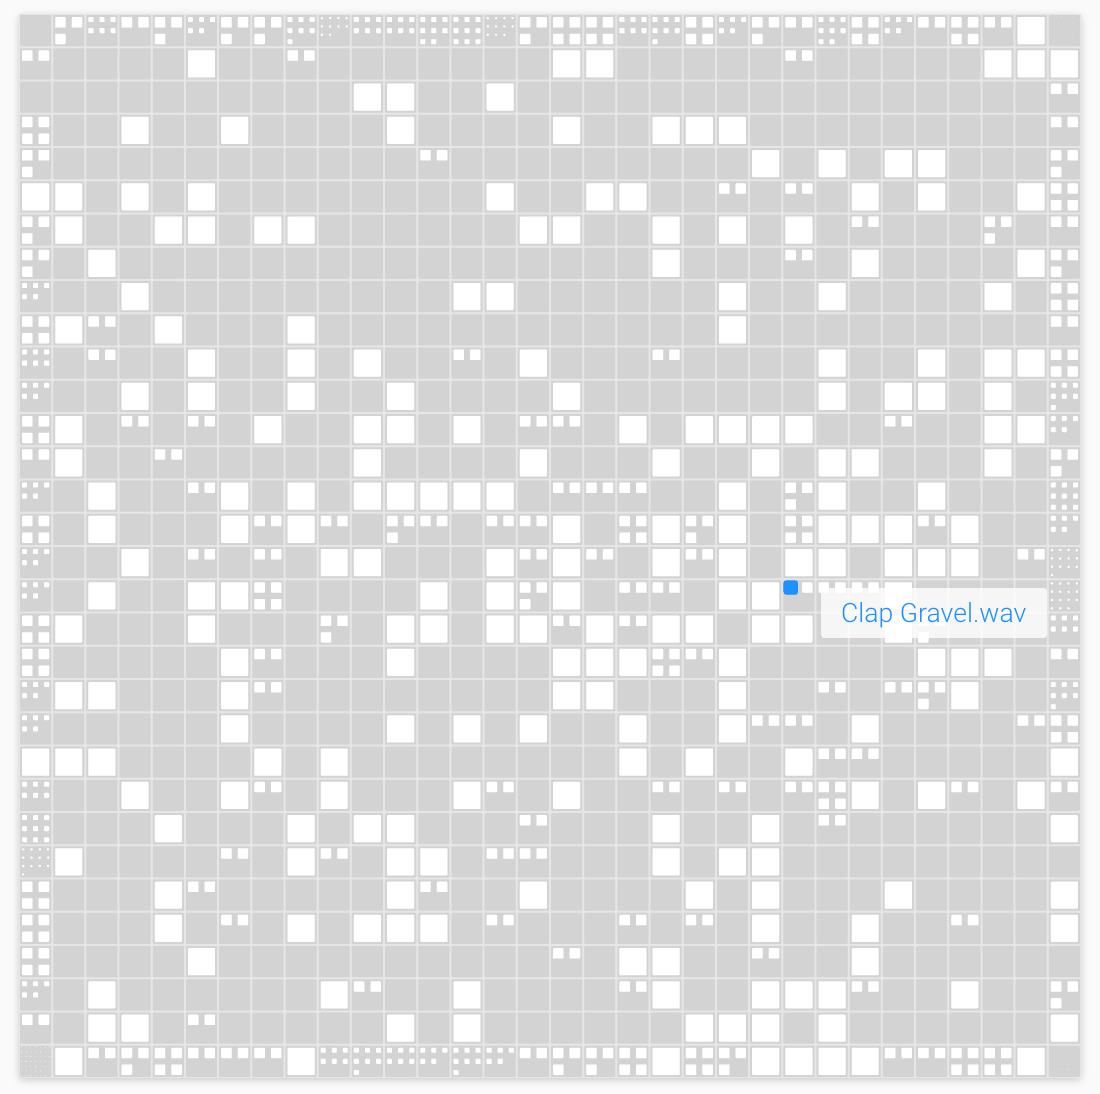
\includegraphics[width=\textwidth]{SOM-Browser_no-FNP}
  \caption{\textit{SOM Browser} without \gls{fnp}}
  \label{fig:results_no_fnp}
\end{subfigure}
~
\begin{subfigure}{0.45\textwidth}
  \centering
  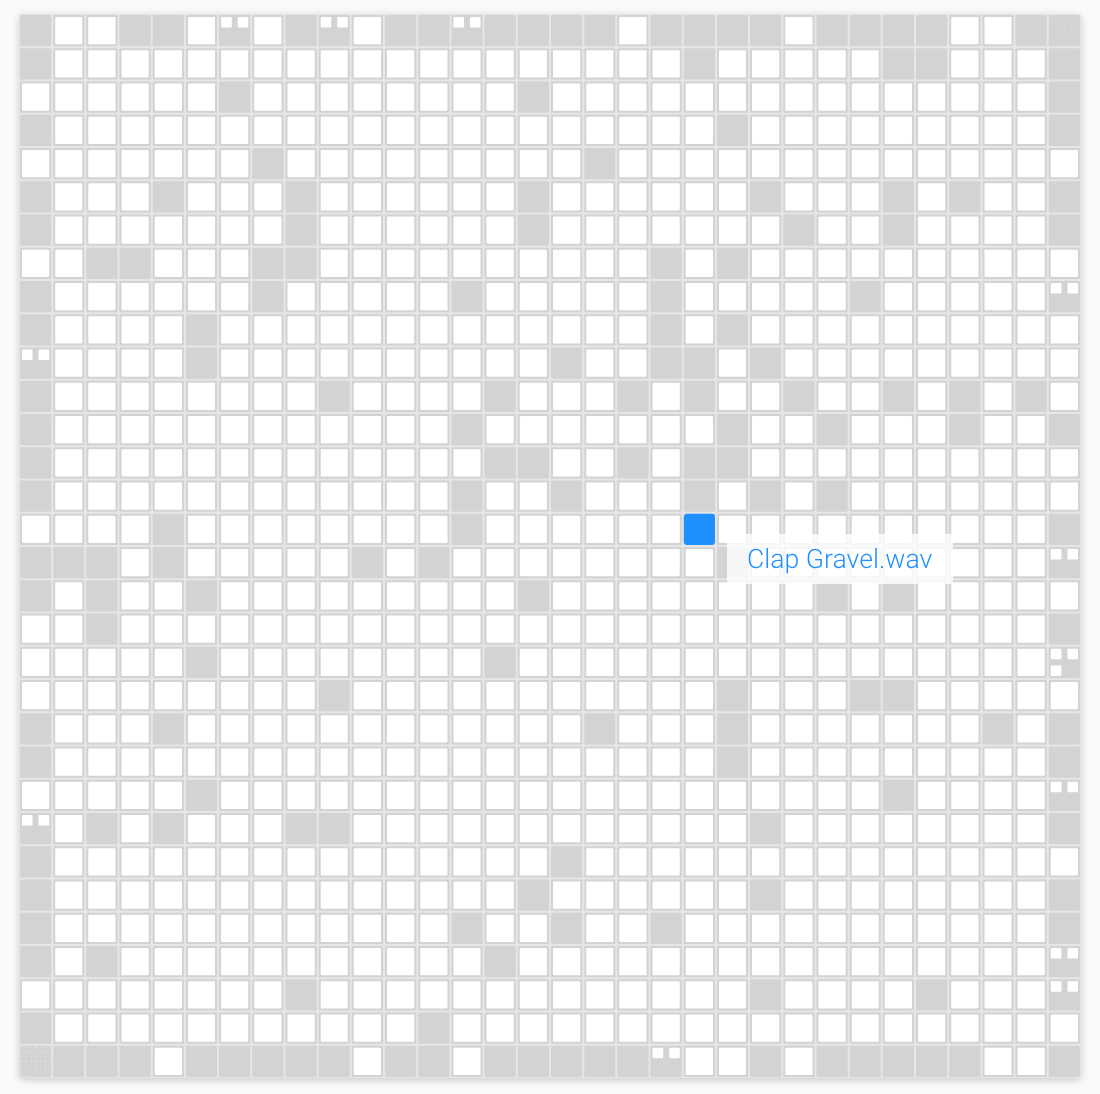
\includegraphics[width=\textwidth]{SOM-Browser_FNP}
  \caption{\textit{SOM Browser} with \gls{fnp}}
  \label{fig:results_fnp}
\end{subfigure}
\caption[\textit{SOM Browser}: Influence of FNP on Map Emptiness]
{\textit{SOM Browser}: Influence of FNP on Map Emptiness for the
\textit{Drum Essentials} sample library}
\label{fig:results_fnp_comparison}
\end{figure}


\subsection{Interview Results}
\label{subsec:results_interview}

Reference grounded theory?

code categories: cognitive, physical, perceptual, strategies, interaction style

phys: arrow keys

perceptual: colors, font size, map order

cognitive: map order, no labelled axes, overwhelming / clear interface

emergent coding vs a priori

Overview Code Tree?

% \begin{figure}[!htb]
%   \centering
% \Tree[.IP [.NP [.Det \textit{the} ]
%                [.N\1 [.N \textit{package} ]]]
%           [.I\1 [.I \textsc{3sg.Pres} ]
%                 [.VP [.V\1 [.V \textit{is} ]
%                            [.AP [.Deg \textit{really} ]
%                                 [.A\1 [.A \textit{simple} ]
%                                       \qroof{\textit{to use}}.CP ]]]]]]
% \caption{A tree caption}
% \label{table:tree_test}
% \end{figure}
%
% \forestset{
%       mathsf content/.style={content
%       format={\noexpand\ensuremath{\noexpand\mathsf{\forestoption{content}}}}},
%       }
%
% \begin{figure}[!htb]
%   \centering
%   \textbf{Established Sample Library Workflow}\par
%   \vspace{0.5cm}
%   \begin{prooftree}
%     {for tree={mathsf content}}
%     {
%       single branches
%     }
%     [, just=explan 1
%       [NP, just=explan 2
%         [Det [the]]
%         [N [cat]]
%       ]
%       [VP
%         [V [sat]]
%         [PP, just=explan 3
%           [P [on]]
%           [NP, just=explan 4
%             [Det, just=explan 5 [the, just=explan 6]]
%             [N [mat]]
%           ]
%         ]
%       ]
%     ]
%   \end{prooftree}
% \caption{A tree caption}
% \label{table:results_current_workflow}
% \end{figure}

\begin{figure}[!htb]
  \centering
  \begin{tikzpicture}[node distance=3mm,
    box/.style={
      rectangle, text centered, rounded corners,
      minimum width = 5cm, minimum height = 2cm,
      fill=table-bg-two, text width=5cm
    },
    item/.style={
      rectangle, text centered, rounded corners, font=\footnotesize,
      minimum width = 3cm, minimum height = 1cm,
      fill=table-bg-two, text width=3cm
    },
    arrow/.style={
      thick,->,>=stealth
    }
  ]
  % \tikzstyle{every node}=[font=\footnotesize]

  \node (well_defined) [item] {Well-Defined};
  \node (ambiguous) [item, below = of well_defined] {Ambiguous};
  \node (os) [item, below = 6mm of ambiguous] {\gls{os} File Browser};
  \node (daw) [item, below = of os] {\gls{daw} Browser};
  \node (sequential) [item, below = 6mm of daw] {Sequential};
  \node (name_based) [item, below = of sequential] {Name-Based};
  \node (random) [item, below = of name_based] {Random};
  \node (match) [item, below = 6mm of random] {Match};
  \node (iteration) [item, below = of match] {Iteration};

  \path (well_defined.west)-- coordinate (aux1) (ambiguous.west);
  \node (mental_representation) [box, left = 6mm of aux1]
  {Mental Representation \\of Sound};

  \path (os.west)-- coordinate (aux2) (daw.west);
  \node (tool) [box, left = 6mm of aux2] {Search Tool};

  \node(algorithm) [box, left = 6mm of name_based] {Search Algorithm};

  \path (match.west)-- coordinate (aux3) (iteration.west);
  \node (evaluation) [box, left = 6mm of aux3] {Contextual Evaluation};

  \draw [arrow] (mental_representation) -- (tool);
  \draw [arrow] (tool) -- (algorithm);
  \draw [arrow] (algorithm) -- (evaluation);

  \draw [arrow] (mental_representation) -- (well_defined);
  \draw [arrow] (mental_representation) -- (ambiguous);

  \draw [arrow] (tool) -- (os);
  \draw [arrow] (tool) -- (daw);

  \draw [arrow] (algorithm) -- (evaluation);
  \draw [arrow] (algorithm) -- (sequential);
  \draw [arrow] (algorithm) -- (name_based);
  \draw [arrow] (algorithm) -- (random);

  \draw [arrow] (evaluation) -- (match);
  \draw [arrow] (evaluation) -- (iteration);

  \node (ctrl1) [below = 1cm of iteration, anchor = south] {};
  \node (ctrl2) [below left = 1cm of evaluation, anchor = north] {};
  \node (ctrl3) [left = 9mm of algorithm, anchor = west] {};
  % HOLY $#&* THIS ARROW WAS A STRUGGLE TO GET STRAIGHT
  \draw [dashed, arrow] (iteration.south) -- (ctrl1.north) -- (ctrl2.east) --
  (ctrl3.east) -- (algorithm);
\end{tikzpicture}
\caption[Established sample library workflow]{Flowchart of established sample
library workflow as described by interview subjects}
\label{table:results_current_workflow}
\end{figure}

cite \citet{saldana2015}

\begin{figure}[!htb]
  \centering
  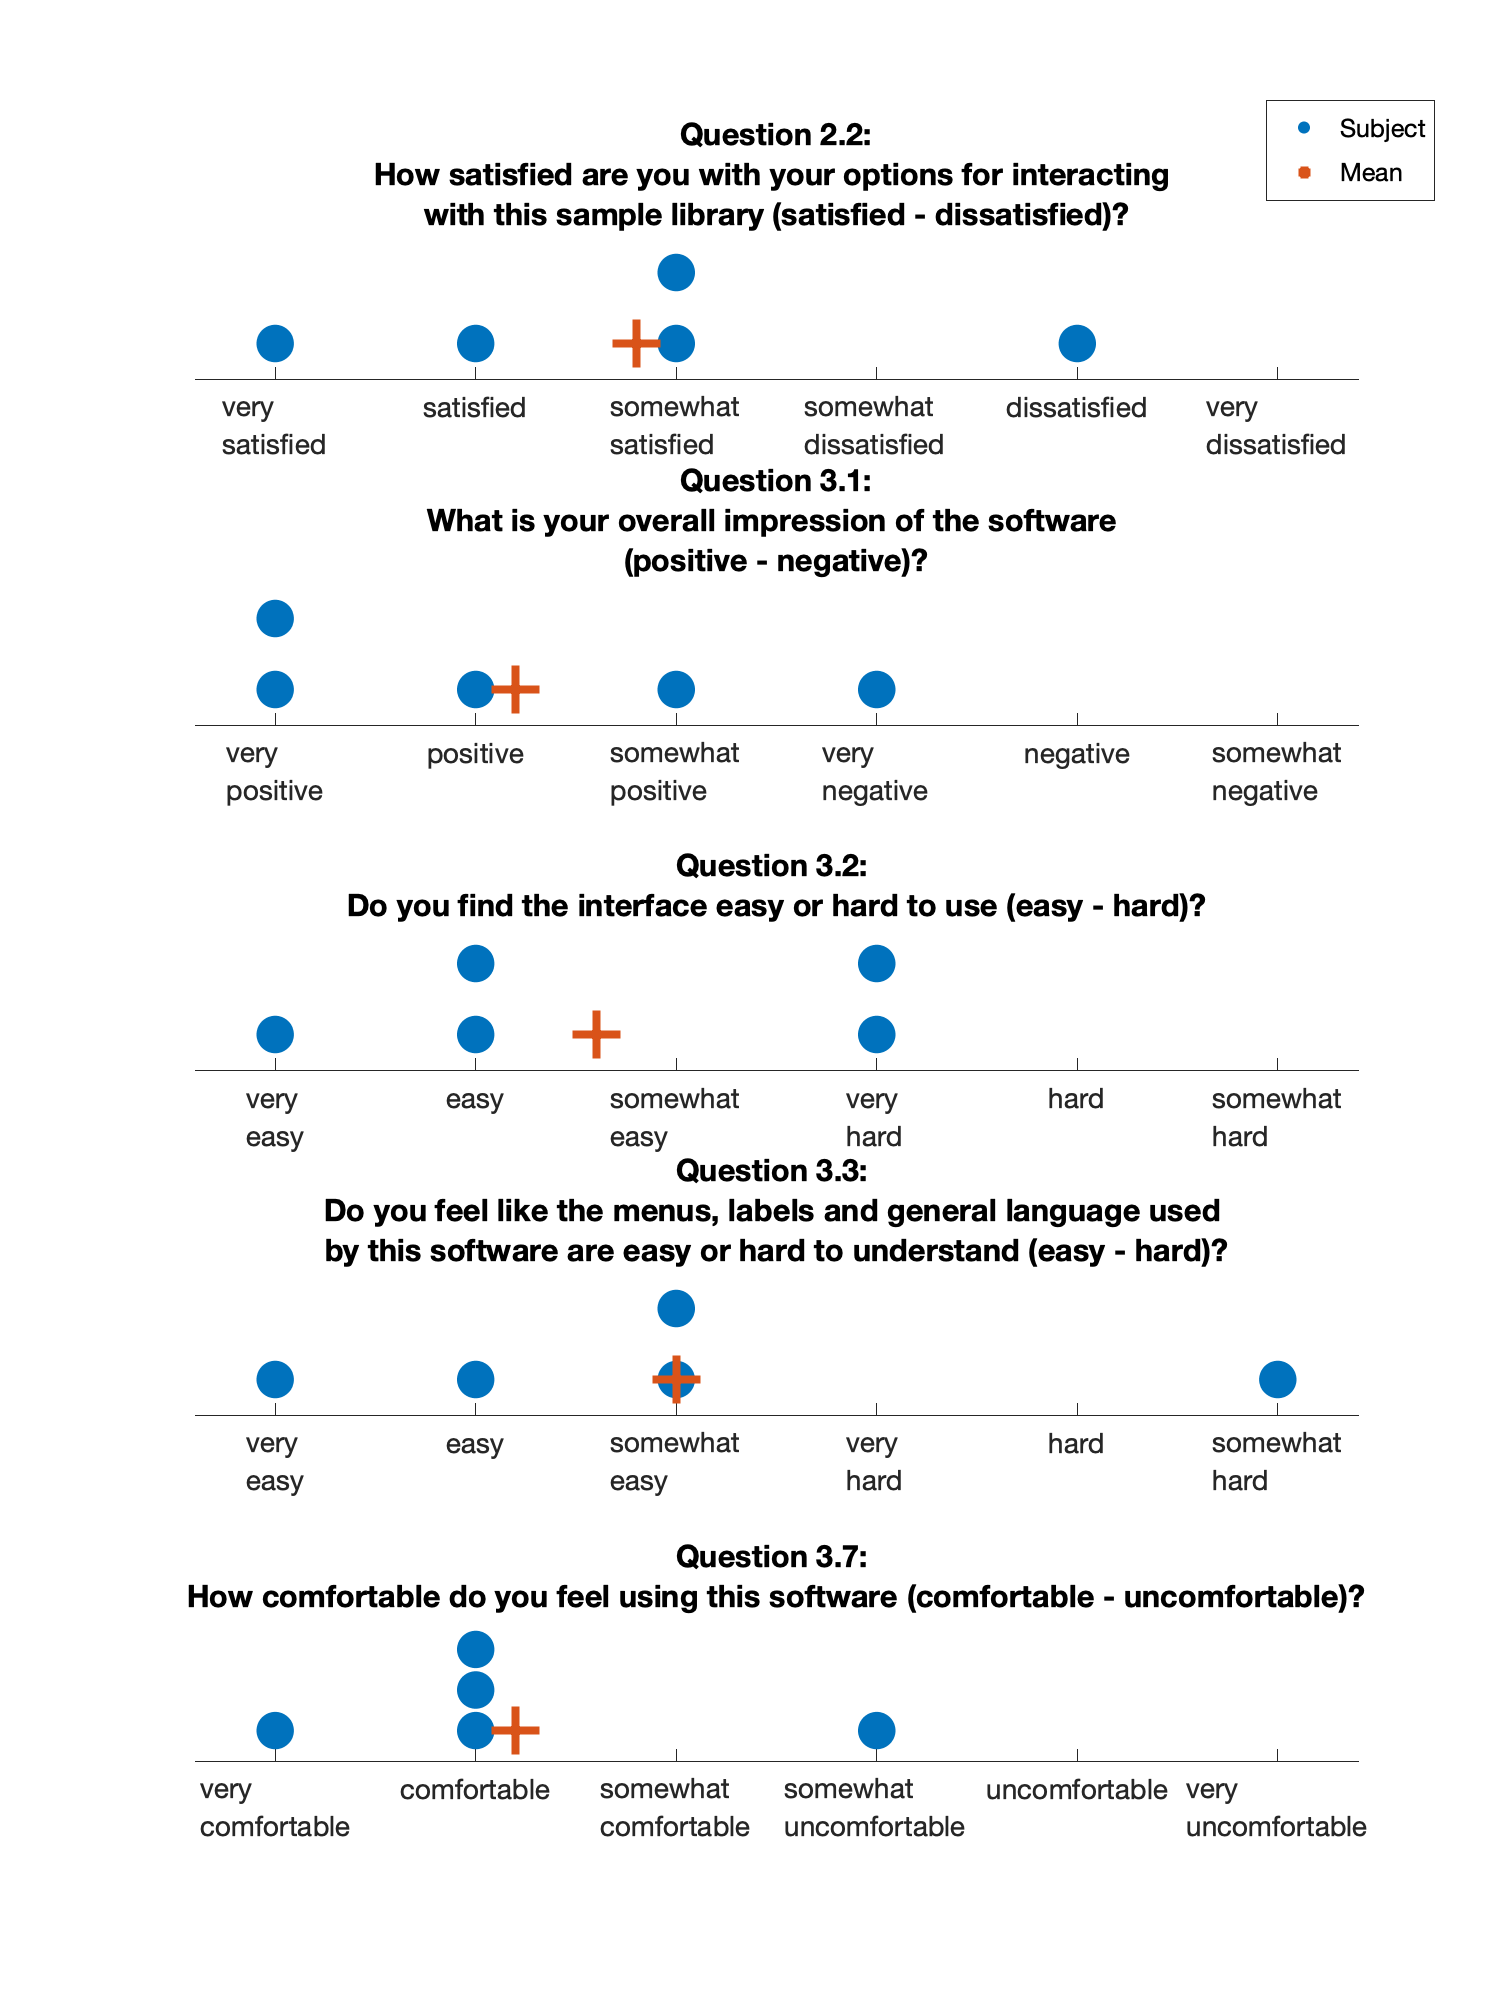
\includegraphics[width=\linewidth, trim = 25mm 10mm 10mm 10mm, clip]
  {eval_ratings}
  \caption[Interview Ratings]{Likert scale ratings by interview subjects for
  questions concerning satisfaction with their current sample library workflow
  and first \textit{SOM Browser} impressions}
  \label{fig:results_ratings}
\end{figure}

\clearpage

\begin{table}[!htb]
  \renewcommand{\arraystretch}{1.2}
  \centering
  \footnotesize
  % \rowcolors{2}{table-bg-one}{table-bg-two}
  \begin{tabular}{ p{4.0cm} p{4.75cm} p{4.75cm} }
  \multicolumn{3}{ l }{\textbf{Question 2.1:}} \\
  \multicolumn{3}{ p{14.5cm} }{\textbf{Imagine you were asked to familiarize
  yourself with the presented sample library in order to use it in some of your
  work. Can you describe how you would approach this task?}} \\
  \hline
    \textbf{Code} & \textbf{Example} & \textbf{Summary} \\
    \hline
    \textbf{Mental Representation}
    &
    "I know exactly what I'm looking for"
    &
    Subjects often have a clear \textbf{mental representation} of the sound they
    are searching.
    \\
    \textbf{Goal Pursuit}
    &
    [I listen to sounds] "[u]ntil I find the one that I want"
    &
    Subjects will only look for sounds until they find something that satisfies
    their immediate needs.
    \\
    \textbf{Search Algorithm}
    &
    "I would just go through every folder [...] and listen carefully to every
    sound"
    &
    Subjects describe three \textbf{search "algorithms"}: sequential
    (listening in alphabetical order), name-based (looking at file or subfolder
    names) and random search (arbitrarily selecting samples).
    \\
    \textbf{Contextual Evaluation}
    &
    "quickly go through the sounds while the track is playing and then find
    one that kind of fits"
    &
    The ability to audition sounds in the \textbf{context} of the relevant
    project is important.
    \\
    \textbf{Iteration}
    &
    "I will have like eight different kick drums [...] and then I go through
    them again as another iteration of choice."
    &
    Subjects will select a variety of samples as potential candidates and then
    perform another search among the selected subset.
    \\
    \textbf{Frustration}
    &
    "it takes a lot of time actually and it's not the most fun part"
    &
    Looking through lists of samples sequentially is perceived to cause
    \textbf{frustration}.
    \\
  \end{tabular}
  \caption[Question 2.1: Response codes]{Question 2.1: Response codes with
  example data and interpretive summary}
  \label{table:responses_question_2-1}
\end{table}

\begin{table}[!ht]
  \renewcommand{\arraystretch}{1.2}
  \centering
  \footnotesize
  % \rowcolors{2}{table-bg-one}{table-bg-two}
  \begin{tabular}{ p{4.0cm} p{4.75cm} p{4.75cm} }
  \multicolumn{3}{ l }{\textbf{Question 2.2:}} \\
  \multicolumn{3}{ p{14.5cm} }{\textbf{How satisfied are you with your options
  for interacting with this sample library?}} \\
  \hline
    \textbf{Code} & \textbf{Example} & \textbf{Summary} \\
    \hline
    \textbf{Requires Organization}
    &
    "if I was organized and I had my 5000 sounds from the past five years it
    [would] be really nice"
    &
    Subjects note that their current workflow relies on sample libraries that
    are organized in some way and note sources of \textbf{frustration} such as
    lost or duplicate files.
    \\
    \textbf{Requires Experience}
    &
    "experience [...] is probably the key"
    &
    \textbf{Experience} (both in a general professional sense and specific to
    the sample libraries at hand) is mentioned as a factor for an efficient,
    successful workflow.
    \\
    \textbf{Good Enough}
    &
    "It could be better but it's okay. Like, it works in most of cases."
    &
    Current workflow practices are deemed \textbf{"good enough"}, but subjects
    are interested in alternative approaches.
    \\
    \textbf{Time-Consuming}
    &
    "[H]ow to listen to all this?"
    &
    Subjects remark upon the amount of time and effort that go into searching
    through sample libraries.
    \\
    \textbf{Overwhelming}
    &
    "it was overwhelming [...] to look through all this"
    &
    Finding relevant samples in a library is described as \textbf{overwhelming}.
    \\
    \textbf{Alphabetic Bias}
    &
    "I think it makes no sense that I'm mainly choosing from the first half of
    the alphabet"
    &
    Sample selection is influenced by alphabetical name ordering. Typically,
    samples positioned towards the beginning of an alphabetical list are more
    likely to be chosen.
    \\
  \end{tabular}
  \caption[Question 2.2: Response codes]{Question 2.2: Response codes with
  example data and interpretive summary}
  \label{table:responses_question_2-2}
\end{table}

\begin{table}[!ht]
  \renewcommand{\arraystretch}{1.2}
  \centering
  \footnotesize
  % \rowcolors{2}{table-bg-one}{table-bg-two}
  \begin{tabular}{ p{4.0cm} p{4.75cm} p{4.75cm} }
  \multicolumn{3}{ l }{\textbf{Question 3.1:}} \\
  \multicolumn{3}{ p{14.5cm} }{\textbf{What is your overall impression of the
  software (positive - negative)? What do you think works or doesn’t work?}} \\
  \hline
    \textbf{Code} & \textbf{Example} & \textbf{Summary} \\
    \hline
    \textbf{Example}
    &
    "Here's an example of something someone said."
    &
    Subjects said this because they believe it to be true.
    \\
  \end{tabular}
  \caption[Question 3.1: Response codes]{Question 3.1: Response codes with
  example data and interpretive summary}
  \label{table:responses_question_3-1}
\end{table}

\begin{table}[!ht]
  \renewcommand{\arraystretch}{1.2}
  \centering
  \footnotesize
  % \rowcolors{2}{table-bg-one}{table-bg-two}
  \begin{tabular}{ p{4.0cm} p{4.75cm} p{4.75cm} }
  \multicolumn{3}{ l }{\textbf{Question 3.2:}} \\
  \multicolumn{3}{ p{14.5cm} }{\textbf{Do you find the interface easy or hard to
  use (easy - hard)? Can you elaborate on why?}} \\
  \hline
    \textbf{Code} & \textbf{Example} & \textbf{Summary} \\
    \hline
    \textbf{Example}
    &
    "Here's an example of something someone said."
    &
    Subjects said this because they believe it to be true.
    \\
  \end{tabular}
  \caption[Question 3.2: Response codes]{Question 3.2: Response codes with example
  data and interpretive summary}
  \label{table:responses_question_3-2}
\end{table}

\begin{table}[!ht]
  \renewcommand{\arraystretch}{1.2}
  \centering
  \footnotesize
  % \rowcolors{2}{table-bg-one}{table-bg-two}
  \begin{tabular}{ p{4.0cm} p{4.75cm} p{4.75cm} }
  \multicolumn{3}{ l }{\textbf{Question 3.3:}} \\
  \multicolumn{3}{ p{14.5cm} }{\textbf{Do you feel like the menus, labels and
  general language used by this software are easy or hard to understand
  (easy - hard)?}} \\
  \hline
    \textbf{Code} & \textbf{Example} & \textbf{Summary} \\
    \hline
    \textbf{Example}
    &
    "Here's an example of something someone said."
    &
    Subjects said this because they believe it to be true.
    \\
  \end{tabular}
  \caption[Question 3.3: Response codes]{Question 3.3: Response codes with
  example data and interpretive summary}
  \label{table:responses_question_3-3}
\end{table}

\begin{table}[!ht]
  \renewcommand{\arraystretch}{1.2}
  \centering
  \footnotesize
  % \rowcolors{2}{table-bg-one}{table-bg-two}
  \begin{tabular}{ p{4.0cm} p{4.75cm} p{4.75cm} }
  \multicolumn{3}{ l }{\textbf{Question 3.4:}} \\
  \multicolumn{3}{ p{14.5cm} }{\textbf{What do you think about the organization
  of sounds in this interface?}} \\
  \hline
    \textbf{Code} & \textbf{Example} & \textbf{Summary} \\
    \hline
    \textbf{Example}
    &
    "Here's an example of something someone said."
    &
    Subjects said this because they believe it to be true.
    \\
  \end{tabular}
  \caption[Question 3.4: Response codes]{Question 3.4: Response codes with
  example
  data and interpretive summary}
  \label{table:responses_question_3-4}
\end{table}

\begin{table}[!ht]
  \renewcommand{\arraystretch}{1.2}
  \centering
  \footnotesize
  % \rowcolors{2}{table-bg-one}{table-bg-two}
  \begin{tabular}{ p{4.0cm} p{4.75cm} p{4.75cm} }
  \multicolumn{3}{ l }{\textbf{Question 3.5:}} \\
  \multicolumn{3}{ p{14.5cm} }{\textbf{What do you think the axes represent?}} \\
  \hline
    \textbf{Code} & \textbf{Example} & \textbf{Summary} \\
    \hline
    \textbf{Example}
    &
    "Here's an example of something someone said."
    &
    Subjects said this because they believe it to be true.
    \\
  \end{tabular}
  \caption[Question 3.5: Response codes]{Question 3.2: Response codes with
  example data and interpretive summary}
  \label{table:responses_question_3-5}
\end{table}

\begin{table}[!ht]
  \renewcommand{\arraystretch}{1.2}
  \centering
  \footnotesize
  % \rowcolors{2}{table-bg-one}{table-bg-two}
  \begin{tabular}{ p{4.0cm} p{4.75cm} p{4.75cm} }
  \multicolumn{3}{ l }{\textbf{Question 3.6:}} \\
  \multicolumn{3}{ p{14.5cm} }{\textbf{Which do you prefer: the map layout or a
  traditional file manager interface and folder structure (or a combination of
  both)?}} \\
  \hline
    \textbf{Code} & \textbf{Example} & \textbf{Summary} \\
    \hline
    \textbf{Example}
    &
    "Here's an example of something someone said."
    &
    Subjects said this because they believe it to be true.
    \\
  \end{tabular}
  \caption[Question 3.6: Response codes]{Question 3.6: Response codes with
  example data and interpretive summary}
  \label{table:responses_question_3-6}
\end{table}

\begin{table}[!ht]
  \renewcommand{\arraystretch}{1.2}
  \centering
  \footnotesize
  % \rowcolors{2}{table-bg-one}{table-bg-two}
  \begin{tabular}{ p{4.0cm} p{4.75cm} p{4.75cm} }
  \multicolumn{3}{ l }{\textbf{Question 3.7:}} \\
  \multicolumn{3}{ p{14.5cm} }{\textbf{How comfortable do you feel using this
  software (comfortable - uncomfortable)?}} \\
  \hline
    \textbf{Code} & \textbf{Example} & \textbf{Summary} \\
    \hline
    \textbf{Example}
    &
    "Here's an example of something someone said."
    &
    Subjects said this because they believe it to be true.
    \\
  \end{tabular}
  \caption[Question 3.7: Response codes]{Question 3.7: Response codes with
  example data and interpretive summary}
  \label{table:responses_question_3-7}
\end{table}

\begin{table}[!ht]
  \renewcommand{\arraystretch}{1.2}
  \centering
  \footnotesize
  % \rowcolors{2}{table-bg-one}{table-bg-two}
  \begin{tabular}{ p{4.0cm} p{4.75cm} p{4.75cm} }
  \multicolumn{3}{ l }{\textbf{Question 3.8:}} \\
  \multicolumn{3}{ p{14.5cm} }{\textbf{Would you consider using this tool in the
  future or not? If not, what changes would you like to see?}} \\
  \hline
    \textbf{Code} & \textbf{Example} & \textbf{Summary} \\
    \hline
    \textbf{Example}
    &
    "Here's an example of something someone said."
    &
    Subjects said this because they believe it to be true.
    \\
  \end{tabular}
  \caption[Question 3.8: Response codes]{Question 3.8: Response codes with
  example data and interpretive summary}
  \label{table:responses_question_3-8}
\end{table}

\cleardoublepage

% !TEX root = ../thesis.tex

\section{Discussion}
\label{sec:discussion}
This is the Discussion.

\subsection{Outlook}
\label{subsec:outlook}

\cleardoublepage

\nocite{*}

\bibliographystyle{FG_AK_English_AuthorYear}
\bibliography{thesis_bib}

\cleardoublepage

\newpage

\cleardoublepage

% !TEX root = ../thesis.tex

\begin{appendices}

All supplementary materials listed here are included with the digital
submission of this work.

\section{Source Code}

The {\LaTeX} sources for this work are located in the directory \texttt{tex/}.

\bigskip

\noindent
The source code for the applications that were developed for this thesis
can be found in the following directories:

\bigskip

\noindent
\textit{mubu-SOM-js}: \quad \texttt{dev/mubu-som-js/}

\bigskip

\noindent
\textit{SOM Browser}: \quad \texttt{dev/som-browser/}

\section{Sample Library}

The \textit{Drum Essentials} sample library that was used as a sound corpus can
be found in \texttt{evaluation/DrumEssentials/}.

\section{Evaluation Map Data}

All maps used for the results presented in Section \ref{sec:results} can be
found in \texttt{evaluation/eval\_maps/}.

\section{Interview Data}

The recorded interviews, their transcriptions and a spreadsheet with the
codified data are located in \texttt{evaluation/interviews/}.

\section{MATLAB Figures}

The MATLAB scripts to create the figures shown in Section \ref{sec:results} can
be found in\\ \texttt{evaluation/matlab/}.


\end{appendices}


\cleardoublepage

\pagenumbering{Roman}
\setcounter{page}{1}
\pagestyle{plain}
\printglossaries
\newpage

\listoffigures
\newpage

\listoflistings
\newpage

\listoftables
\newpage

\phantomsection
\addcontentsline{toc}{section}{Digital Resource}
\section*{Digital Resource}
\label{digital_resource}
\vspace{23em}
\centering
\scriptsize
This page holds a data disk.
\newpage

\end{document}
